\documentclass[12pt]{article}

% ---------- Paquetes ----------
\usepackage[utf8]{inputenc}
\usepackage[T1]{fontenc}
\usepackage[spanish]{babel}
\usepackage{graphicx}
\usepackage{hyperref}

%\usepackage[margin=1in]{geometry}
\usepackage{amsmath,amsthm,amssymb}
\usepackage{braket}
\usepackage{graphicx}

\usepackage[dvipsnames]{xcolor}
\usepackage[margin=2.5cm]{geometry}
\usepackage{subcaption}
\usepackage{booktabs}
\usepackage{listings}


% ---------- Tipografía: EB Garamond (si está instalada) ----------
%\IfFileExists{ebgaramond.sty}{\usepackage{ebgaramond}}{\usepackage{mathpazo}}
\IfFileExists{lmodern.sty}{\usepackage{lmodern}}{}

% ---------- Color del logo de la UAM ----------
%\definecolor{uamazul}{RGB}{0,114,206}


\newcommand{\N}{\mathbb{N}}
\newcommand{\R}{\mathbb{R}}
\newcommand{\Z}{\mathbb{Z}}
\newcommand{\Q}{\mathbb{Q}}

% ---------- Datos del documento ----------
%\title{Práctica 2: Algoritmos cuánticos básicos con Qiskit}
%\author{Zhengkai Zhu\\ 
%        Marco López Borrego}
%\date{}


\addto\captionsspanish{\renewcommand{\tablename}{Tabla}}

%\setcounter{secnumdepth}{0}
\newcounter{savedsecnumdepth}


\begin{document}

% ---------- Portada ----------
% ============================================================
%  Portada
%  Coloca el logo en imagenes/logo_uam.png (si no existe se
%  muestra un texto azul de sustitución).
% ============================================================

% ---- Datos de la portada (edita aquí) ----
\newcommand{\PortadaTitulo}{Práctica 2: Algoritmos cuánticos básicos con Qiskit}
\newcommand{\PortadaMaster}{Máster en Computación Cuántica}
\newcommand{\PortadaAsignatura}{Laboratorio de Computación en Circuitos cuánticos}
\newcommand{\PortadaCurso}{Curso 2026-2027}

\begin{titlepage}
  \centering
  \vspace*{0.5cm}

  % ---- Logo ----
  \IfFileExists{imagenes/Logo_UAM.jpg}{%
    
\includegraphics[width=0.45\textwidth]{imagenes/Logo_UAM.jpg}%
  }{%
    {\color{uamazul}\Huge\bfseries UAM}\\[2pt]
    {\color{uamazul}\Large Universidad Autónoma\\de Madrid}%
  }

  \vspace{2cm}

  % ---- Título ----
  {\fontsize{24}{32}\selectfont\bfseries \PortadaTitulo\par}

  \vspace{2cm}

  % ---- Máster, asignatura y curso ----
  {\Large\bfseries \PortadaMaster\par}
  \vspace{4pt}
  {\large\itshape \PortadaAsignatura\par}
  \vspace{8pt}
  {\large \PortadaCurso\par}

  \vspace{2.2cm}

  % ---- Alumnos ----
  {\large\bfseries Alumnos\par}
  \vspace{4pt}
  {\normalsize Zhengkai Zhu\par}
  {\normalsize Marco López Borrego\par}

  \vfill
\end{titlepage}



\tableofcontents
\newpage

% ---------- Secciones (cada una en su propio fichero) ----------
%\section{Objetivos}\label{sec:objetivos}

En esta práctica se realizan ejercicios experimentales que sirven de introducción a los algoritmos
cuánticos. A lo largo de ella se adquieren y afianzan conceptos básicos de algoritmia cuántica y se
implementan, con Qiskit, soluciones a los problemas planteados en el enunciado.

Sobre la base de los conocimientos de programación en Qiskit ya consolidados, se construyen los circuitos
de los algoritmos cuánticos y se realizan simulaciones para comparar los resultados experimentales con
las predicciones teóricas.

Los objetivos concretos son:
\begin{itemize}
    \item Estudiar e implementar oráculos cuánticos reversibles a partir de funciones booleanas.
    \item Analizar el efecto de \textbf{retroceso de fase} (\textit{phase kickback}) y su relación con los oráculos de fase.
    \item Implementar y analizar los algoritmos de consulta \textbf{Deutsch}, \\
    \textbf{Deutsch-Jozsa} y \textbf{Bernstein-Vazirani}.
    \item Implementar y analizar el \textbf{algoritmo de Grover}, incluido el número óptimo de iteraciones.
    \item Implementar la \textbf{estimación cuántica de fase (QPE)} de un operador $U$ sobre un autovector $\ket{\psi}$.
    \item Contrastar en cada caso los resultados simulados con los teóricos.
\end{itemize}
%\section{Entorno de trabajo y convenciones}\label{sec:entorno_convenciones}

Esta sección recoge el software y los simuladores empleados, y las convenciones de notación que se siguen en toda la memoria, indicando de forma explícita
los casos en los que un bloque se aparta de la convención general.

%--------------------------------------------------------------------
\subsection{Entorno de trabajo}\label{subsec:entorno}

\begin{itemize}
    \item \textbf{Software.} Python 3.12.3 en un cuaderno Jupyter, con \texttt{qiskit} (versión \texttt{2.6.1}), \\
    \texttt{qiskit-aer} (versión \texttt{0.18.2}),
    \texttt{numpy}, \texttt{scipy} (test $\chi^2$), \texttt{matplotlib} y \texttt{tabulate}. % COMPLETAR: sustituir X.Y.Z con qiskit.__version__ y qiskit_aer.__version__
    \item \textbf{Histogramas de medida.} Se usa \texttt{AerSimulator()} con $4096$ disparos (\textit{shots}), salvo que se indique otra cosa en el ejercicio.
    Se elige porque el resultado pedido es una medida: simula el muestreo estadístico de un circuito con medidas, incluido el caso de un único disparo.
    \item \textbf{Vectores de estado y matrices.} Para las amplitudes en un punto intermedio del circuito se usa \texttt{Statevector} sobre el circuito \emph{sin medidas}, y
    \texttt{Operator} para comparar matrices de circuitos. Se eligen porque dan las amplitudes y fases exactas, que una medida no permite recuperar
    (por ejemplo, las fases relativas de los Bloques 2 y 5).
    \item \textbf{Aleatoriedad.} Los conteos de los Bloques 1, 2 y 4 se obtienen con la semilla del simulador fijada (\texttt{seed\_simulator} $=98$), por lo que son
    reproducibles bit a bit. En los Bloques 3 y 5 no se fija la semilla del simulador, de modo que los conteos exactos pueden variar ligeramente entre ejecuciones,
    aunque los resultados cualitativos (por ejemplo, las medidas deterministas) no cambian.
    % Si se añade seed_simulator=seed en los Bloques 3 y 5 y se vuelve a ejecutar, sustituir la última frase por:
    % "Todos los conteos de la memoria se obtienen con la semilla del simulador fijada (\texttt{seed\_simulator} $=98$) y son reproducibles."
    \item \textbf{Comparación teoría--simulación.} Los histogramas se contrastan con la predicción teórica; cuando se indica, mediante un test $\chi^2$ de bondad de ajuste
    con nivel de significación del $5\%$ (el resultado es compatible con la teoría si $p>0{,}05$). Con $4096$ disparos, el ruido estadístico típico de una
    probabilidad es $\sim1/\sqrt{4096}\approx0{,}016$.
\end{itemize}

La Tabla~\ref{tab:entorno_simuladores} resume qué simulador se ha usado en cada bloque.

\begin{table}[htbp]
    \centering
    \begin{tabular}{c|p{0.4\textwidth}|p{0.35\textwidth}}
    \hline
    Bloque & \texttt{AerSimulator} (medidas) & \texttt{Statevector} / \texttt{Operator} (amplitudes) \\
    \hline
    1 & Tablas de verdad e histogramas (disparos) & Predicción en superposición; verificación $U_f^2=I$ \\
    2 & Probabilidades de medir $q_0$; tabla de verdad de $U_f$ & Estados tras cada puerta, esferas de Bloch, autovalores $\lambda$ \\
    3 & Histogramas de Deutsch, Deutsch-Jozsa y Bernstein-Vazirani (un solo disparo en BV) & --- \\
    4 & Histogramas de Grover y $P_k$ simulada & Amplitudes $a_i$, $b_i$ y $P_k$ exacta \\
    5 & Histogramas de QPE & Estados en los puntos 1--3 del circuito (E2.1) \\
    \hline
    \end{tabular}
    \caption{Simulador empleado en cada bloque y motivo de su uso.}\label{tab:entorno_simuladores}
\end{table}

%--------------------------------------------------------------------
\subsection{Convenciones de notación}\label{subsec:convenciones}

\paragraph{Orden de los bits (\textit{little-endian}).} Qiskit usa el convenio \textit{little-endian}: el qubit $q_0$ es el menos significativo. Un estado de $n$ qubits se escribe
$|q_{n-1}\dots q_1q_0\rangle$ y corresponde al elemento de índice $\sum_j q_j2^j$ del vector de estado. Al medir con la asignación habitual $q_j\to c_j$, la cadena de
medida es $c_{n-1}\dots c_1c_0$: el bit de la \emph{derecha} es el del qubit $q_0$. En los oráculos, la variable de entrada $x_j$ vive en el qubit $q_j$ y el bit
$f_j$ de la salida se suma (XOR) al qubit $q_{n+j}$, por lo que la cadena medida se lee $f_{m-1}\dots f_0\,x_{n-1}\dots x_0$ (salida a la izquierda, entrada a la derecha).

\paragraph{Fases.} Como se pide en el enunciado, la fase de un autovalor se escribe $\lambda=e^{2\pi i\theta}$ con $\theta\in[0,1)$, es decir, en \emph{fracciones de vuelta}.
La puerta de fase $P(\varphi)=\mathrm{diag}(1,e^{i\varphi})$ se parametriza con el ángulo $\varphi$ en radianes, por lo que su fase en fracciones de vuelta es $\theta=\varphi/2\pi$
(por ejemplo, $P(\pi/2)$ tiene $\theta=1/4$). En QPE con $t$ qubits de conteo, si se mide $m$, la fase estimada es $\tilde\varphi=m/2^t$ y el error es $|\tilde\varphi-\theta|$.

\paragraph{Esfera de Bloch.} Los vectores de Bloch se calculan a partir de los valores esperados $(\langle X\rangle,\langle Y\rangle,\langle Z\rangle)$ de cada qubit, lo que
sigue siendo válido cuando el qubit está entrelazado con otros. La fase relativa de un qubit se ve como un giro alrededor del eje $z$; una fase global no se ve.

\paragraph{Probabilidades.} Las probabilidades simuladas son las frecuencias relativas $\text{conteo}/\text{shots}$, y los histogramas se muestran en conteos
(número de disparos) salvo que se indique lo contrario.

\paragraph{Convenciones de cada bloque y excepciones.} La Tabla~\ref{tab:entorno_convenios} indica la correspondencia entre variables, qubits y bits de la cadena medida
en cada bloque. Los Bloques 1, 2 y 4 siguen la convención general sin excepciones. Las particularidades están en los Bloques 3 y 5.

\begin{table}[htbp]
    \centering
    {\small\setlength{\tabcolsep}{4pt}
    \begin{tabular}{c|p{0.30\textwidth}|p{0.22\textwidth}|p{0.28\textwidth}}
    \hline
    Bloque & Variables y qubits & Asignación de medida & Cadena medida \\
    \hline
    1 & $x_j\to q_j$; $f_j\to q_{n+j}$ & $q_j\to c_j$ & $f_{m-1}\dots f_0\,x_{n-1}\dots x_0$ \\
    2 & Dato $x\equiv q_0$, ancilla $y\equiv q_1$ (2.5); control $q_0$ y objetivo $q_1$ & $q_j\to c_j$ & $q_1q_0$ \\
    3.1, 3.2 & Deutsch: dato $q_0$, ancilla $q_1$. Deutsch-Jozsa ($n=2$): $f(x_1,x_0)$, $x_j\to q_j$, ancilla $q_2$ & $q_j\to c_j$ & $q_1q_0$ (datos) \\
    3.3 y E1 & \textbf{Orden inverso:} la clave $a$ y la entrada se escriben con el bit de $q_0$ a la izquierda: $a=a_0a_1a_2a_3$; $f(x_0,x_1)$ & \textbf{Invertida:} $q_j\to c_{n-1-j}$ & Se lee $q_0q_1\dots q_{n-1}$ \\
    4 & $w=x_{n-1}\dots x_0$, $x_j\to q_j$; $|w\rangle$ es el índice $\mathrm{int}(w,2)$ & $q_j\to c_j$ & $c_{n-1}\dots c_0$ \\
    5 & Registro de conteo en $q_0\dots q_{t-1}$; autovector en $q_t$; el qubit de conteo $j$ controla $U^{2^j}$ & $q_j\to c_j$ & $c_{t-1}\dots c_0$ ($=m$ en binario) \\
    \hline
    \end{tabular}}
    \caption{Correspondencia entre variables, qubits y cadena de medida en cada bloque.}\label{tab:entorno_convenios}
\end{table}

\subsubsection*{Bloque 3: Bernstein-Vazirani y ejercicio E1 (orden inverso)}
En el ejercicio 3.3 el oráculo de la clave oculta se construye escribiendo $a$ con el bit de $q_0$ a la izquierda, es decir $a=a_0a_1a_2a_3$ y una puerta CNOT desde
cada $q_j$ con $a_j=1$ hacia la ancilla $q_4$. Por ejemplo, para $a=1010$ hay CNOT desde $q_0$ y $q_2$, y para $a=1101$ desde $q_0$, $q_1$ y $q_3$. Esta notación es la contraria
a la de Qiskit (y a la del ejercicio 1.6, donde $a=a_4\dots a_0$). Para que la cadena medida se lea igual que la clave se invierte la asignación de bits clásicos,
\texttt{measure(range(4), range(3, -1, -1))}, es decir $q_j\to c_{3-j}$, de forma que la cadena $c_3c_2c_1c_0$ se lee $q_0q_1q_2q_3$. De manera análoga, en el ejercicio E1
la función se escribe $f(x_0,x_1)$ con $q_0$ primero, y se mide con \texttt{measure([0, 1], [1, 0])}, de modo que la cadena $|q_0q_1\rangle$ se lee con $q_0$ a la izquierda
y la tabla de verdad se ordena con $x=2x_0+x_1$. En el ejercicio 3.2 (Deutsch-Jozsa con $n=2$) \emph{no} se invierte: $f(x_1,x_0)$ y la cadena medida es $c_1c_0=x_1x_0$.

\subsubsection*{Bloque 5: QPE}
En QPE el registro de conteo ocupa los qubits $q_0,\dots,q_{t-1}$ y el autovector el qubit $q_t$. El qubit de conteo $j$ controla $U^{2^j}$ y a continuación se aplica la
$\mathrm{QFT}^\dagger$ (\texttt{QFTGate(t).inverse()}) sobre el registro de conteo. La medida usa la asignación estándar $q_j\to c_j$ (\texttt{measure(range(t), range(t))}),
sin inversión: la cadena $c_{t-1}\dots c_0$ es directamente la representación binaria de $m$, con $q_{t-1}$ como bit más significativo, y la fase estimada es $\tilde\varphi=m/2^t$.
Los estados del sistema completo se escriben con el autovector a la izquierda, $|{\psi_{\text{autovector}}}\rangle\otimes|{\text{registro de conteo}}\rangle$; por ejemplo,
en E2.1 ($t=3$) el ket $|1000\rangle$ corresponde a $q_3=1$ y $q_2q_1q_0=000$. Cuando se mide también el qubit del autovector (E2.4~c), este es el bit clásico más
significativo de la cadena, $c_tc_{t-1}\dots c_0$.

\setcounter{savedsecnumdepth}{\value{secnumdepth}}         % guarda el valor de tu clase
\setcounter{secnumdepth}{0}
\section{Objetivos}\label{sec:objetivos}

En esta práctica se realizan ejercicios experimentales que sirven de introducción a los algoritmos
cuánticos. A lo largo de ella se adquieren y afianzan conceptos básicos de algoritmia cuántica y se
implementan, con Qiskit, soluciones a los problemas planteados en el enunciado.

Sobre la base de los conocimientos de programación en Qiskit ya consolidados, se construyen los circuitos
de los algoritmos cuánticos y se realizan simulaciones para comparar los resultados experimentales con
las predicciones teóricas.

Los objetivos concretos son:
\begin{itemize}
    \item Estudiar e implementar oráculos cuánticos reversibles a partir de funciones booleanas.
    \item Analizar el efecto de \textbf{retroceso de fase} (\textit{phase kickback}) y su relación con los oráculos de fase.
    \item Implementar y analizar los algoritmos de consulta \textbf{Deutsch}, \\
    \textbf{Deutsch-Jozsa} y \textbf{Bernstein-Vazirani}.
    \item Implementar y analizar el \textbf{algoritmo de Grover}, incluido el número óptimo de iteraciones.
    \item Implementar la \textbf{estimación cuántica de fase (QPE)} de un operador $U$ sobre un autovector $\ket{\psi}$.
    \item Contrastar en cada caso los resultados simulados con los teóricos.
\end{itemize}                                          % o tu \section{Objetivos}
\section{Entorno de trabajo y convenciones}\label{sec:entorno_convenciones}

Esta sección recoge el software y los simuladores empleados, y las convenciones de notación que se siguen en toda la memoria, indicando de forma explícita
los casos en los que un bloque se aparta de la convención general.

%--------------------------------------------------------------------
\subsection{Entorno de trabajo}\label{subsec:entorno}

\begin{itemize}
    \item \textbf{Software.} Python 3.12.3 en un cuaderno Jupyter, con \texttt{qiskit} (versión \texttt{2.6.1}), \\
    \texttt{qiskit-aer} (versión \texttt{0.18.2}),
    \texttt{numpy}, \texttt{scipy} (test $\chi^2$), \texttt{matplotlib} y \texttt{tabulate}. % COMPLETAR: sustituir X.Y.Z con qiskit.__version__ y qiskit_aer.__version__
    \item \textbf{Histogramas de medida.} Se usa \texttt{AerSimulator()} con $4096$ disparos (\textit{shots}), salvo que se indique otra cosa en el ejercicio.
    Se elige porque el resultado pedido es una medida: simula el muestreo estadístico de un circuito con medidas, incluido el caso de un único disparo.
    \item \textbf{Vectores de estado y matrices.} Para las amplitudes en un punto intermedio del circuito se usa \texttt{Statevector} sobre el circuito \emph{sin medidas}, y
    \texttt{Operator} para comparar matrices de circuitos. Se eligen porque dan las amplitudes y fases exactas, que una medida no permite recuperar
    (por ejemplo, las fases relativas de los Bloques 2 y 5).
    \item \textbf{Aleatoriedad.} Los conteos de los Bloques 1, 2 y 4 se obtienen con la semilla del simulador fijada (\texttt{seed\_simulator} $=98$), por lo que son
    reproducibles bit a bit. En los Bloques 3 y 5 no se fija la semilla del simulador, de modo que los conteos exactos pueden variar ligeramente entre ejecuciones,
    aunque los resultados cualitativos (por ejemplo, las medidas deterministas) no cambian.
    % Si se añade seed_simulator=seed en los Bloques 3 y 5 y se vuelve a ejecutar, sustituir la última frase por:
    % "Todos los conteos de la memoria se obtienen con la semilla del simulador fijada (\texttt{seed\_simulator} $=98$) y son reproducibles."
    \item \textbf{Comparación teoría--simulación.} Los histogramas se contrastan con la predicción teórica; cuando se indica, mediante un test $\chi^2$ de bondad de ajuste
    con nivel de significación del $5\%$ (el resultado es compatible con la teoría si $p>0{,}05$). Con $4096$ disparos, el ruido estadístico típico de una
    probabilidad es $\sim1/\sqrt{4096}\approx0{,}016$.
\end{itemize}

La Tabla~\ref{tab:entorno_simuladores} resume qué simulador se ha usado en cada bloque.

\begin{table}[htbp]
    \centering
    \begin{tabular}{c|p{0.4\textwidth}|p{0.35\textwidth}}
    \hline
    Bloque & \texttt{AerSimulator} (medidas) & \texttt{Statevector} / \texttt{Operator} (amplitudes) \\
    \hline
    1 & Tablas de verdad e histogramas (disparos) & Predicción en superposición; verificación $U_f^2=I$ \\
    2 & Probabilidades de medir $q_0$; tabla de verdad de $U_f$ & Estados tras cada puerta, esferas de Bloch, autovalores $\lambda$ \\
    3 & Histogramas de Deutsch, Deutsch-Jozsa y Bernstein-Vazirani (un solo disparo en BV) & --- \\
    4 & Histogramas de Grover y $P_k$ simulada & Amplitudes $a_i$, $b_i$ y $P_k$ exacta \\
    5 & Histogramas de QPE & Estados en los puntos 1--3 del circuito (E2.1) \\
    \hline
    \end{tabular}
    \caption{Simulador empleado en cada bloque y motivo de su uso.}\label{tab:entorno_simuladores}
\end{table}

%--------------------------------------------------------------------
\subsection{Convenciones de notación}\label{subsec:convenciones}

\paragraph{Orden de los bits (\textit{little-endian}).} Qiskit usa el convenio \textit{little-endian}: el qubit $q_0$ es el menos significativo. Un estado de $n$ qubits se escribe
$|q_{n-1}\dots q_1q_0\rangle$ y corresponde al elemento de índice $\sum_j q_j2^j$ del vector de estado. Al medir con la asignación habitual $q_j\to c_j$, la cadena de
medida es $c_{n-1}\dots c_1c_0$: el bit de la \emph{derecha} es el del qubit $q_0$. En los oráculos, la variable de entrada $x_j$ vive en el qubit $q_j$ y el bit
$f_j$ de la salida se suma (XOR) al qubit $q_{n+j}$, por lo que la cadena medida se lee $f_{m-1}\dots f_0\,x_{n-1}\dots x_0$ (salida a la izquierda, entrada a la derecha).

\paragraph{Fases.} Como se pide en el enunciado, la fase de un autovalor se escribe $\lambda=e^{2\pi i\theta}$ con $\theta\in[0,1)$, es decir, en \emph{fracciones de vuelta}.
La puerta de fase $P(\varphi)=\mathrm{diag}(1,e^{i\varphi})$ se parametriza con el ángulo $\varphi$ en radianes, por lo que su fase en fracciones de vuelta es $\theta=\varphi/2\pi$
(por ejemplo, $P(\pi/2)$ tiene $\theta=1/4$). En QPE con $t$ qubits de conteo, si se mide $m$, la fase estimada es $\tilde\varphi=m/2^t$ y el error es $|\tilde\varphi-\theta|$.

\paragraph{Esfera de Bloch.} Los vectores de Bloch se calculan a partir de los valores esperados $(\langle X\rangle,\langle Y\rangle,\langle Z\rangle)$ de cada qubit, lo que
sigue siendo válido cuando el qubit está entrelazado con otros. La fase relativa de un qubit se ve como un giro alrededor del eje $z$; una fase global no se ve.

\paragraph{Probabilidades.} Las probabilidades simuladas son las frecuencias relativas $\text{conteo}/\text{shots}$, y los histogramas se muestran en conteos
(número de disparos) salvo que se indique lo contrario.

\paragraph{Convenciones de cada bloque y excepciones.} La Tabla~\ref{tab:entorno_convenios} indica la correspondencia entre variables, qubits y bits de la cadena medida
en cada bloque. Los Bloques 1, 2 y 4 siguen la convención general sin excepciones. Las particularidades están en los Bloques 3 y 5.

\begin{table}[htbp]
    \centering
    {\small\setlength{\tabcolsep}{4pt}
    \begin{tabular}{c|p{0.30\textwidth}|p{0.22\textwidth}|p{0.28\textwidth}}
    \hline
    Bloque & Variables y qubits & Asignación de medida & Cadena medida \\
    \hline
    1 & $x_j\to q_j$; $f_j\to q_{n+j}$ & $q_j\to c_j$ & $f_{m-1}\dots f_0\,x_{n-1}\dots x_0$ \\
    2 & Dato $x\equiv q_0$, ancilla $y\equiv q_1$ (2.5); control $q_0$ y objetivo $q_1$ & $q_j\to c_j$ & $q_1q_0$ \\
    3.1, 3.2 & Deutsch: dato $q_0$, ancilla $q_1$. Deutsch-Jozsa ($n=2$): $f(x_1,x_0)$, $x_j\to q_j$, ancilla $q_2$ & $q_j\to c_j$ & $q_1q_0$ (datos) \\
    3.3 y E1 & \textbf{Orden inverso:} la clave $a$ y la entrada se escriben con el bit de $q_0$ a la izquierda: $a=a_0a_1a_2a_3$; $f(x_0,x_1)$ & \textbf{Invertida:} $q_j\to c_{n-1-j}$ & Se lee $q_0q_1\dots q_{n-1}$ \\
    4 & $w=x_{n-1}\dots x_0$, $x_j\to q_j$; $|w\rangle$ es el índice $\mathrm{int}(w,2)$ & $q_j\to c_j$ & $c_{n-1}\dots c_0$ \\
    5 & Registro de conteo en $q_0\dots q_{t-1}$; autovector en $q_t$; el qubit de conteo $j$ controla $U^{2^j}$ & $q_j\to c_j$ & $c_{t-1}\dots c_0$ ($=m$ en binario) \\
    \hline
    \end{tabular}}
    \caption{Correspondencia entre variables, qubits y cadena de medida en cada bloque.}\label{tab:entorno_convenios}
\end{table}

\subsubsection*{Bloque 3: Bernstein-Vazirani y ejercicio E1 (orden inverso)}
En el ejercicio 3.3 el oráculo de la clave oculta se construye escribiendo $a$ con el bit de $q_0$ a la izquierda, es decir $a=a_0a_1a_2a_3$ y una puerta CNOT desde
cada $q_j$ con $a_j=1$ hacia la ancilla $q_4$. Por ejemplo, para $a=1010$ hay CNOT desde $q_0$ y $q_2$, y para $a=1101$ desde $q_0$, $q_1$ y $q_3$. Esta notación es la contraria
a la de Qiskit (y a la del ejercicio 1.6, donde $a=a_4\dots a_0$). Para que la cadena medida se lea igual que la clave se invierte la asignación de bits clásicos,
\texttt{measure(range(4), range(3, -1, -1))}, es decir $q_j\to c_{3-j}$, de forma que la cadena $c_3c_2c_1c_0$ se lee $q_0q_1q_2q_3$. De manera análoga, en el ejercicio E1
la función se escribe $f(x_0,x_1)$ con $q_0$ primero, y se mide con \texttt{measure([0, 1], [1, 0])}, de modo que la cadena $|q_0q_1\rangle$ se lee con $q_0$ a la izquierda
y la tabla de verdad se ordena con $x=2x_0+x_1$. En el ejercicio 3.2 (Deutsch-Jozsa con $n=2$) \emph{no} se invierte: $f(x_1,x_0)$ y la cadena medida es $c_1c_0=x_1x_0$.

\subsubsection*{Bloque 5: QPE}
En QPE el registro de conteo ocupa los qubits $q_0,\dots,q_{t-1}$ y el autovector el qubit $q_t$. El qubit de conteo $j$ controla $U^{2^j}$ y a continuación se aplica la
$\mathrm{QFT}^\dagger$ (\texttt{QFTGate(t).inverse()}) sobre el registro de conteo. La medida usa la asignación estándar $q_j\to c_j$ (\texttt{measure(range(t), range(t))}),
sin inversión: la cadena $c_{t-1}\dots c_0$ es directamente la representación binaria de $m$, con $q_{t-1}$ como bit más significativo, y la fase estimada es $\tilde\varphi=m/2^t$.
Los estados del sistema completo se escriben con el autovector a la izquierda, $|{\psi_{\text{autovector}}}\rangle\otimes|{\text{registro de conteo}}\rangle$; por ejemplo,
en E2.1 ($t=3$) el ket $|1000\rangle$ corresponde a $q_3=1$ y $q_2q_1q_0=000$. Cuando se mide también el qubit del autovector (E2.4~c), este es el bit clásico más
significativo de la cadena, $c_tc_{t-1}\dots c_0$.

\setcounter{secnumdepth}{\value{savedsecnumdepth}} 
\section{Bloque 1. Computacion reversible y oráculos booleanos}\label{sec:bloque_1}
\subsection{Ejercicio 1.1. Puerta AND reversible}
Se implementa $|a_1a_0\rangle|0\rangle \to |a_1a_0\rangle|a_1\wedge a_0\rangle$ con una puerta Toffoli: controles
en $q_0\equiv a_0$ y $q_1\equiv a_1$, objetivo en la ancilla $q_2\equiv y$, inicializada a $|0\rangle$.
Cada entrada clásica se prepara con puertas $X$ y se miden los tres qubits; la cadena medida es \texttt{y a1 a0} ($c_2c_1c_0$).

\textbf{Predicción.} La tabla de verdad del AND con las entradas intactas. Como el circuito es determinista,
cada entrada debe dar un único resultado con probabilidad 1.

La puerta Toffoli se muestra en la Figura~\ref{fig:bloque1_e1_1_andtoffoli}.
\begin{figure}[h]
    \centering
    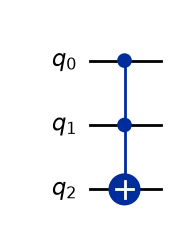
\includegraphics[width=0.15\textwidth]{imagenes/bloque1/e1_1_andtoffoli.png}
    \caption{Puerta Toffoli.}\label{fig:bloque1_e1_1_andtoffoli}
\end{figure}

\begin{figure}[htbp]
    \centering
    \begin{subfigure}{0.4\textwidth}
        \centering
        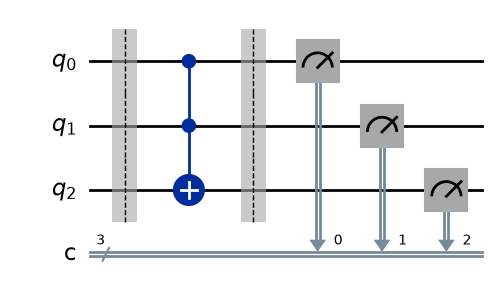
\includegraphics[width=\textwidth]{imagenes/bloque1/e1_1_caso00.png}
        \caption{}
    \end{subfigure}
    \hfill
    \begin{subfigure}{0.4\textwidth}
        \centering
        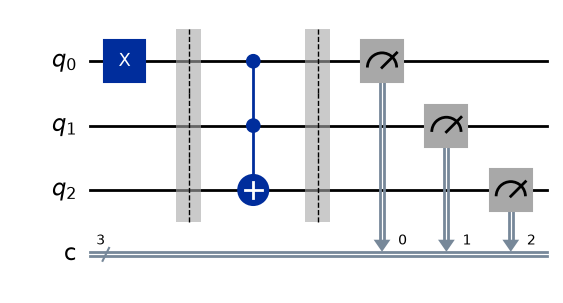
\includegraphics[width=\textwidth]{imagenes/bloque1/e1_1_caso01.png}
        \caption{}
    \end{subfigure}
    \hfill
    \begin{subfigure}{0.4\textwidth}
        \centering
        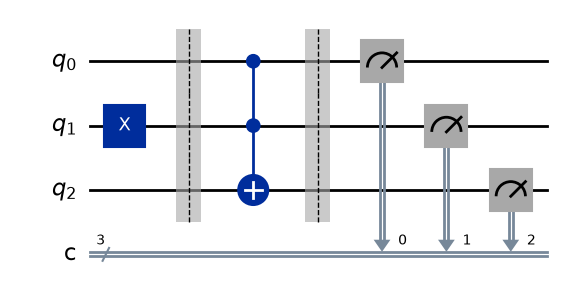
\includegraphics[width=\textwidth]{imagenes/bloque1/e1_1_caso10.png}
        \caption{}
    \end{subfigure}
    \hfill
    \begin{subfigure}{0.4\textwidth}
        \centering
        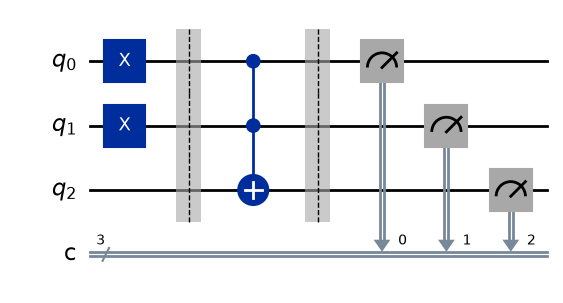
\includegraphics[width=\textwidth]{imagenes/bloque1/e1_1_caso11.png}
        \caption{}
    \end{subfigure}
    \caption{Circuitos de puerta $AND$ para entradas $q_1, q_0 = 00, 01, 10, 11$.}\label{fig:bloque1_e1_1_circuitos}
\end{figure}

La Tabla~\ref{tab:bloque1_e1_1} recoge la tabla de verdad simulada junto a la teórica.

\begin{table}[htbp]
    \centering
\begin{tabular}{c|c|c|c|c}
\hline
$a_1a_0$ & $f(x)$ teórica & $f(x)$ simulada & $x$ tras $U_f$ & Prob. \\
\hline
\texttt{00} & \texttt{0} & \texttt{0} & \texttt{00} & 1 \\
\texttt{01} & \texttt{0} & \texttt{0} & \texttt{01} & 1 \\
\texttt{10} & \texttt{0} & \texttt{0} & \texttt{10} & 1 \\
\texttt{11} & \texttt{1} & \texttt{1} & \texttt{11} & 1 \\
\hline
\end{tabular}
    \caption{Ejercicio 1.1: tabla de verdad del AND reversible. La columna $x$ tras $U_f$ es la entrada medida después del oráculo.}\label{tab:bloque1_e1_1}
\end{table}

\textbf{Resultado.} Para las cuatro entradas la salida medida coincide con la tabla de verdad del AND ($y=1$ únicamente para $a_1a_0=11$),
con probabilidad 1 y sin ningún otro resultado. Los qubits de entrada se miden exactamente en el estado en que se prepararon: el oráculo conserva la entrada
y escribe $f(a)$ en la ancilla mediante una suma módulo 2, y eso es lo que hace reversible un AND (que por sí solo no lo es, ya que a partir de la salida no se pueden
recuperar las entradas). La matriz del circuito coincide con la permutación $|x\rangle|y\rangle\mapsto|x\rangle|y\oplus f(x)\rangle$ y cumple $U_f^2=I$.

%--------------------------------------------------------------------
\subsection{Ejercicio 1.2. Paralelismo cuántico}

Se aplican puertas $H$ a $q_0$ y $q_1$ para preparar $\tfrac12(|00\rangle+|01\rangle+|10\rangle+|11\rangle)|0\rangle$ y después el oráculo. Por linealidad:

$$U_f\Big(\tfrac12\sum_{a_1a_0}|a_1a_0\rangle\Big)|0\rangle=\tfrac12\big(|00\rangle|0\rangle+|01\rangle|0\rangle+|10\rangle|0\rangle+|11\rangle|1\rangle\big).$$

En la Figura~\ref{fig:bloque1_e1_2_circuito} se muestra el circuito correspondiente.

\begin{figure}[h]
     \centering
    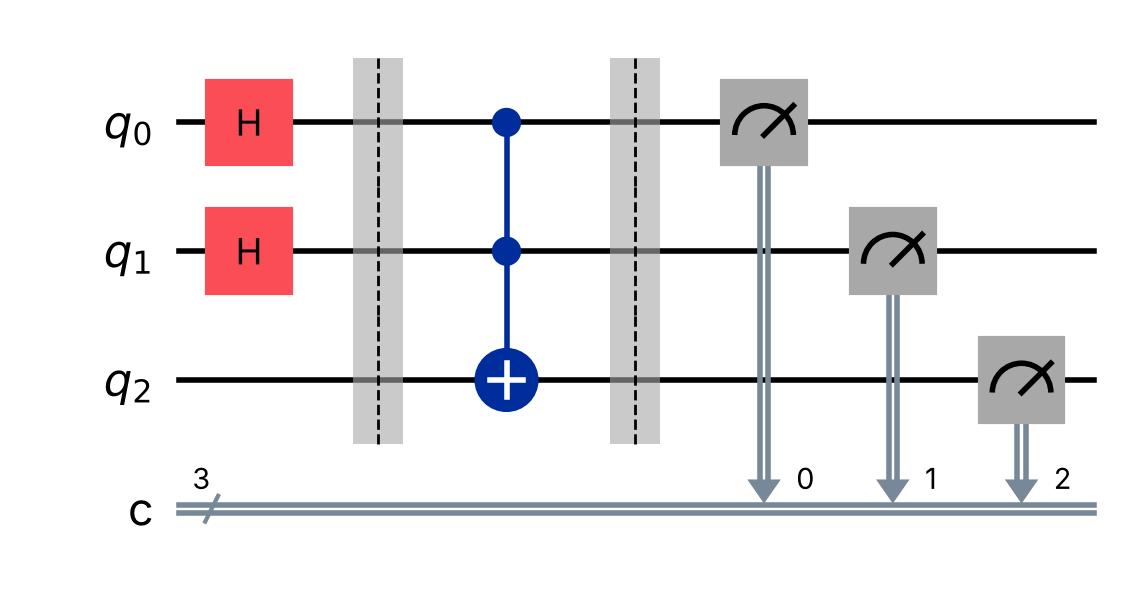
\includegraphics[width=0.5\textwidth]{imagenes/bloque1/e1_2_circuito.png}
    \caption{Circuito completo.}\label{fig:bloque1_e1_2_circuito}
\end{figure}

\textbf{Predicción.} Al medir los tres qubits aparecen cuatro cadenas \texttt{y a1 a0}: \texttt{000}, \texttt{001}, \texttt{010} y \texttt{111},
cada una con probabilidad $1/4$. Se obtiene el estado teórico con \texttt{Statevector} (circuito sin medidas) y se compara con el histograma simulado con \texttt{AerSimulator}
mediante un test $\chi^2$ de bondad de ajuste.

\begin{figure}[htbp]
    \centering
    \begin{subfigure}{0.48\textwidth}
        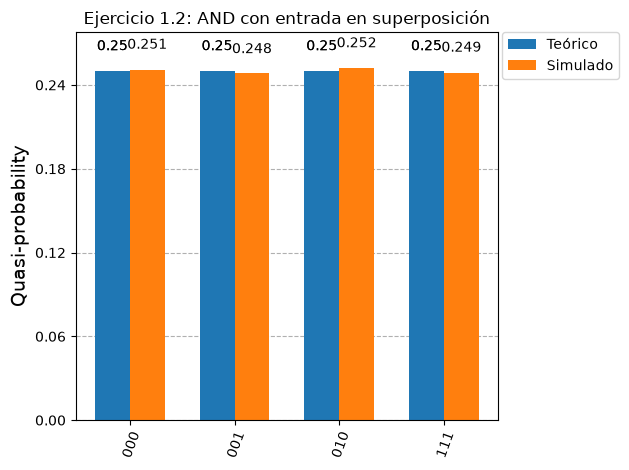
\includegraphics[width=0.9\textwidth]{imagenes/bloque1/e1_2_comp_prediccionTeoria.png}
        \caption{}
    \end{subfigure}
    \hfill
    \begin{subfigure}{0.48\textwidth}
        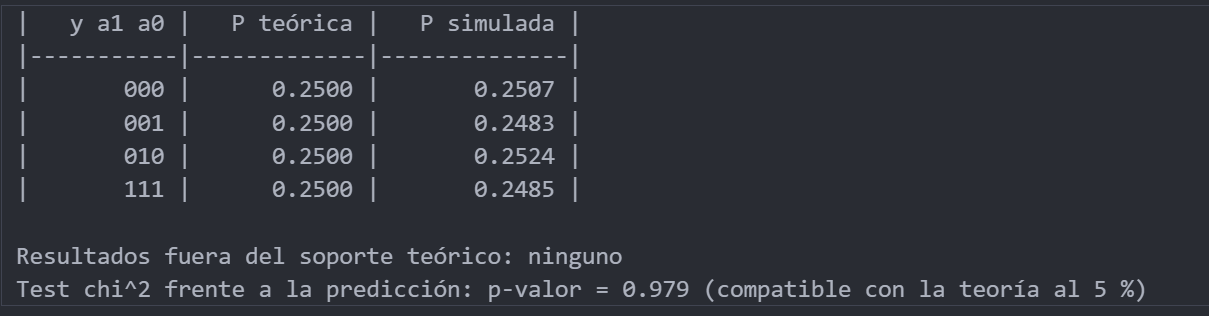
\includegraphics[width=0.9\textwidth]{imagenes/bloque1/e1_2_tabla_comparacion.png}
        \caption{}
    \end{subfigure}
    \caption{(a): Comparación de los histogramas de la predicción teórica y de la simulación.\\
    (b): Tabla comparativa de las probabilidades teóricas y de simulación, con ajuste positivo de $\chi^2$.}\label{fig:bloque1_e1_2_comparacion}
\end{figure}

En la Figura~\ref{fig:bloque1_e1_2_comparacion} se observa que las probabilidades obtenidas en la simulación son prácticamente idénticas a las
teóricas, con pequeñas desviaciones. En el test $\chi^2$ de bondad de ajuste frente a la predicción teórica se obtiene un $p$-valor de $0{,}979$,
compatible con la teoría al $5\%$: las discrepancias entre los datos observados y los predichos son muy pequeñas y
encajan con las fluctuaciones estadísticas esperables con 4096 disparos.

\textbf{¿Y con un solo disparo?} Para comprobarlo experimentalmente se ejecuta el circuito con \emph{un único disparo} en diez ocasiones
independientes (cambiando la semilla del simulador en cada una) y se anota la fila \texttt{y a1 a0} obtenida. En todas las ejecuciones se
obtiene una única fila, distinta de una ejecución a otra, y tras las diez ejecuciones se han visto tres de las cuatro filas posibles: ninguna ejecución
individual da la tabla completa. Después se almacena el resultado de cada disparo de una misma tanda y se cuenta cuántas filas distintas se han observado
tras $k$ disparos (Figura~\ref{fig:bloque1_e1_2_experimento}, izquierda): en la tanda de 40 disparos la tabla se completa en el disparo número 5, no antes.

\begin{figure}[htbp]
    \centering
    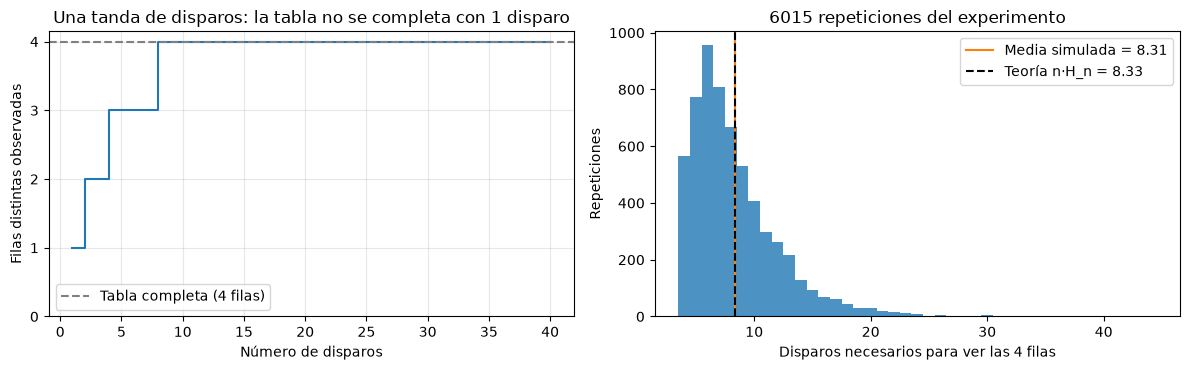
\includegraphics[width=\textwidth]{imagenes/bloque1/e1_2_experimento_1_disparo.png}
    \caption{Experimento de un solo disparo en el ejercicio 1.2.
    Izquierda: filas distintas observadas en función del número de disparos en una tanda; la curva parte de una sola fila y necesita varios disparos para llegar a las cuatro.
    Derecha: histograma del número de disparos necesarios para observar las cuatro filas, repitiendo el experimento 6034 veces; la media simulada ($8{,}29$)
    coincide con la teórica $nH_n=25/3\approx 8{,}33$.}\label{fig:bloque1_e1_2_experimento}
\end{figure}

El histograma de la derecha de la Figura~\ref{fig:bloque1_e1_2_experimento} muestra que el mínimo número de disparos necesarios es 4 y que la distribución tiene una cola larga hacia la derecha
(en algunas repeticiones se necesitan más de 20 disparos). Incluso con exactamente 4 disparos solo se obtiene la tabla completa con probabilidad
$4!/4^4=24/256\approx 9{,}4\%$ (en la simulación, un $9{,}8\%$), mientras que con un solo disparo esa probabilidad es exactamente 0.

%--------------------------------------------------------------------
\subsection{Ejercicio 1.3. Puerta XOR reversible}
Se repiten los ejercicios 1.1 y 1.2 para $f(a_1,a_0)=a_1\oplus a_0$, que se implementa con dos CNOT que comparten objetivo (la ancilla $q_2$):
\texttt{cx(0,2)} y \texttt{cx(1,2)}. El oráculo se muestra en la Figura~\ref{fig:bloque1_e1_3_xor}.

\begin{figure}[h]
    \centering
    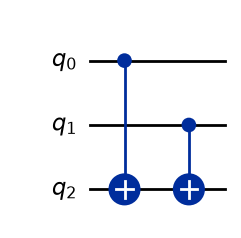
\includegraphics[width=0.3\textwidth]{imagenes/bloque1/e1_3_xor.png}
    \caption{Oráculo XOR reversible con dos puertas CNOT.}\label{fig:bloque1_e1_3_xor}
\end{figure}

\textbf{Predicción con entradas clásicas.} La tabla de verdad del XOR, con las entradas intactas y un único resultado con probabilidad 1 para cada una.

\textbf{Predicción con entrada en superposición.}
$$U_f\Big(\tfrac12\sum_{a_1a_0}|a_1a_0\rangle\Big)|0\rangle=\tfrac12\big(|00\rangle|0\rangle+|01\rangle|1\rangle+|10\rangle|1\rangle+|11\rangle|0\rangle\big),$$
es decir, las cadenas \texttt{y a1 a0} = \texttt{000}, \texttt{101}, \texttt{110} y \texttt{011}, cada una con probabilidad $1/4$.

\begin{figure}[htbp]
    \centering
    \begin{subfigure}{0.4\textwidth}
        \centering
        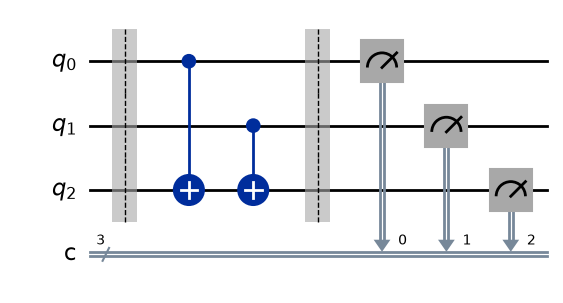
\includegraphics[width=\textwidth]{imagenes/bloque1/e1_3_circuito00.png}
        \caption{}
    \end{subfigure}
    \hfill
    \begin{subfigure}{0.4\textwidth}
        \centering
        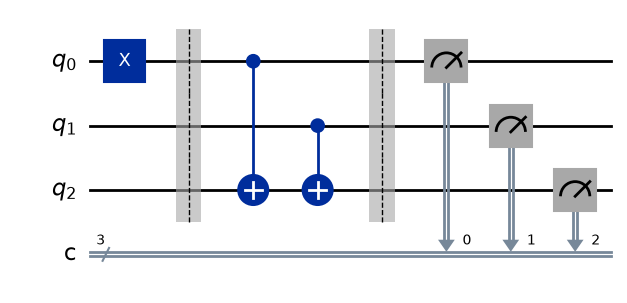
\includegraphics[width=\textwidth]{imagenes/bloque1/e1_3_circuito01.png}
        \caption{}
    \end{subfigure}
    \hfill
    \begin{subfigure}{0.4\textwidth}
        \centering
        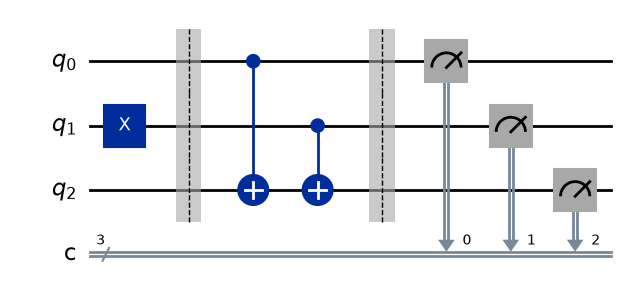
\includegraphics[width=\textwidth]{imagenes/bloque1/e1_3_circuito10.png}
        \caption{}
    \end{subfigure}
    \hfill
    \begin{subfigure}{0.4\textwidth}
        \centering
        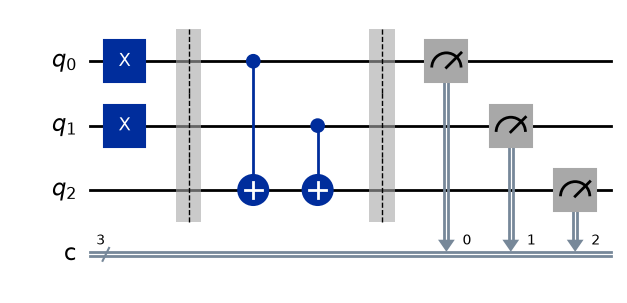
\includegraphics[width=\textwidth]{imagenes/bloque1/e1_3_circuito11.png}
        \caption{}
    \end{subfigure}
    \caption{Circuitos de puerta $XOR$ para entradas $q_1, q_0 = 00, 01, 10, 11$.}\label{fig:bloque1_e1_3_circuitos}
\end{figure}

\begin{table}[htbp]
    \centering
\begin{tabular}{c|c|c|c|c}
\hline
$a_1a_0$ & $f(x)$ teórica & $f(x)$ simulada & $x$ tras $U_f$ & Prob. \\
\hline
\texttt{00} & \texttt{0} & \texttt{0} & \texttt{00} & 1 \\
\texttt{01} & \texttt{1} & \texttt{1} & \texttt{01} & 1 \\
\texttt{10} & \texttt{1} & \texttt{1} & \texttt{10} & 1 \\
\texttt{11} & \texttt{0} & \texttt{0} & \texttt{11} & 1 \\
\hline
\end{tabular}
    \caption{Ejercicio 1.3: tabla de verdad del XOR reversible.}\label{tab:bloque1_e1_3}
\end{table}

La Tabla~\ref{tab:bloque1_e1_3} muestra que, para las cuatro entradas clásicas, la salida simulada coincide con la tabla de verdad del XOR con probabilidad 1 y que
la entrada no se modifica. Con la entrada en superposición se utiliza el circuito de la Figura~\ref{fig:bloque1_e1_3_super} y se compara la distribución
medida con la predicha (Figura~\ref{fig:bloque1_e1_3_comparacion}).

\begin{figure}[h]
    \centering
    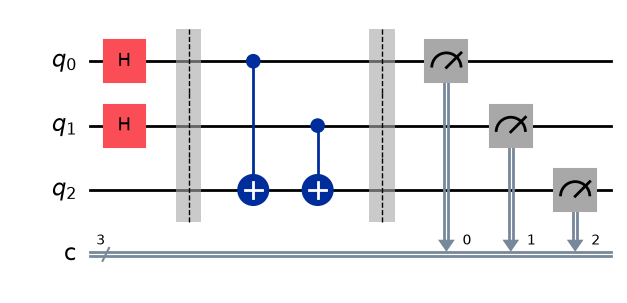
\includegraphics[width=0.5\textwidth]{imagenes/bloque1/e1_3_circuitoXOR_super.png}
    \caption{Circuito XOR con las entradas en superposición.}\label{fig:bloque1_e1_3_super}
\end{figure}

\begin{figure}[h]
    \centering
    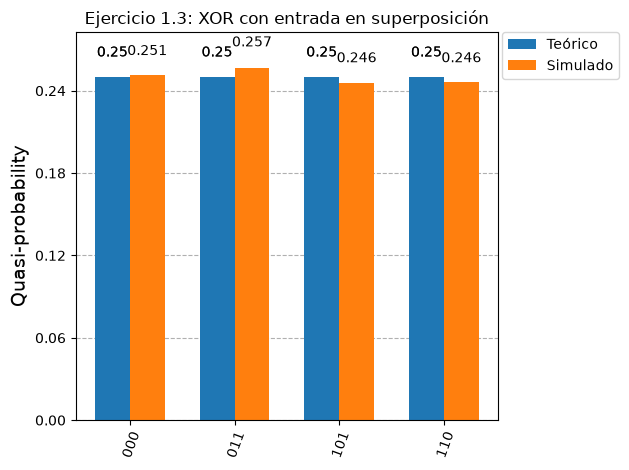
\includegraphics[width=0.6\textwidth]{imagenes/bloque1/e1_3_prediccion_teoria.png}
    \caption{Ejercicio 1.3: comparación entre la predicción teórica y la simulación con la entrada en superposición.}\label{fig:bloque1_e1_3_comparacion}
\end{figure}

\begin{table}[h]
    \centering
    \begin{tabular}{c|c|c}
    \hline
    \texttt{y a1 a0} & $P$ teórica & $P$ simulada \\
    \hline
    \texttt{000} & 0,2500 & 0,2512 \\
    \texttt{011} & 0,2500 & 0,2568 \\
    \texttt{101} & 0,2500 & 0,2456 \\
    \texttt{110} & 0,2500 & 0,2463 \\
    \hline
    \end{tabular}
    \caption{Ejercicio 1.3: probabilidades teóricas y simuladas con entrada en superposición.}\label{tab:bloque1_e1_3_super}
\end{table}


\textbf{¿Y con un solo disparo?} Se repite el experimento del ejercicio 1.2 con el oráculo XOR. Cada ejecución del circuito con un único disparo devuelve
\emph{una sola} fila \texttt{y a1 a0}, elegida al azar entre las cuatro posibles (\texttt{000}, \texttt{011}, \texttt{101} y \texttt{110}), por lo que una
ejecución individual no puede dar la tabla de verdad completa. Para cuantificarlo se almacena el resultado de cada disparo de una misma tanda y se cuenta cuántas filas distintas se han
observado tras $k$ disparos (Figura~\ref{fig:bloque1_e1_3_experimento}, izquierda): en la tanda de 40 disparos la tabla se completa en el disparo número 5, no antes.

\begin{figure}[htbp]
    \centering
    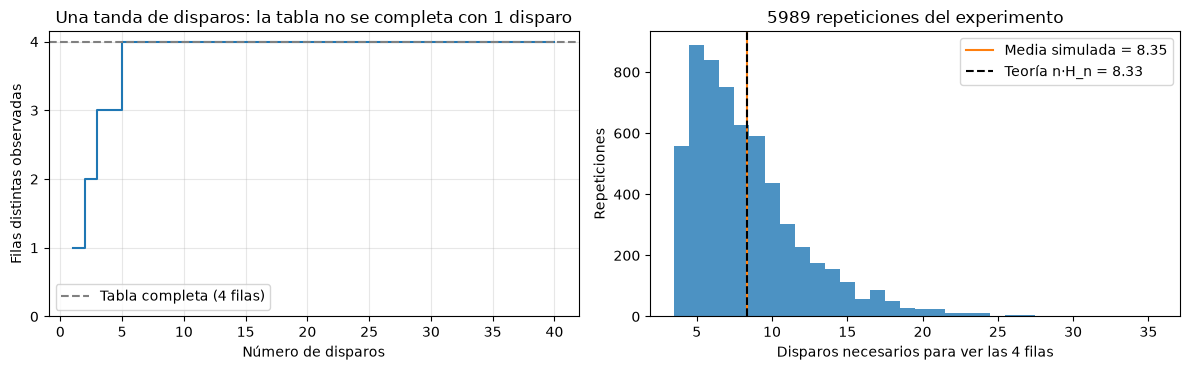
\includegraphics[width=\textwidth]{imagenes/bloque1/e1_3_experimento_1_disparo.png}
    \caption{Experimento de un solo disparo en el ejercicio 1.3 (XOR).
    Izquierda: filas distintas observadas en función del número de disparos en una tanda; la curva parte de una sola fila y necesita varios disparos para llegar a las cuatro.
    Derecha: histograma del número de disparos necesarios para observar las cuatro filas, repitiendo el experimento 5989 veces; la media simulada ($8{,}35$)
    coincide con la teórica $nH_n=25/3\approx 8{,}33$.}\label{fig:bloque1_e1_3_experimento}
\end{figure}

El histograma de la derecha de la Figura~\ref{fig:bloque1_e1_3_experimento} muestra que el mínimo número de disparos necesarios es 4 y que la distribución presenta una cola larga hacia la derecha
(en algunas repeticiones se necesitan más de 20 disparos, e incluso más de 30). Incluso con exactamente 4 disparos solo se obtiene la tabla completa con probabilidad
$4!/4^4=24/256\approx 9{,}4\%$, mientras que con un solo disparo esa probabilidad es exactamente 0. Los resultados son los mismos que con el AND del ejercicio 1.2, como cabe esperar:
el número de disparos necesarios depende solo de que las cuatro filas sean equiprobables, no de la función $f$ implementada.

\textbf{Resultado.} La simulación reproduce las cuatro cadenas previstas con probabilidad $\approx 1/4$ cada una y ninguna otra (Tabla~\ref{tab:bloque1_e1_3_super});
el test $\chi^2$ da un $p$-valor de $0{,}723$, compatible con la teoría al $5\%$. Cada disparo devuelve una sola fila $(a,f(a))$, por lo que un único disparo no da la tabla completa:
hacen falta en media $8{,}35$ disparos para observar las cuatro filas, en excelente acuerdo con el valor teórico $25/3\approx8{,}33$.

Obsérvese que esta $f$ vale 0 en dos entradas y 1 en las otras dos, es decir, es \emph{balanceada}, mientras que el AND del ejercicio 1.1 no lo es.
Esta distinción es la que aprovechará el algoritmo de Deutsch-Jozsa en el Bloque~3.

%--------------------------------------------------------------------
\subsection{Ejercicio 1.4. Oráculo de 3 bits con puertas multicontroladas}
La función vale 1 solo en tres entradas, por lo que basta una puerta multicontrolada por minitérmino ($x_2x_1x_0\in\{001,\,101,\,111\}$), todas con objetivo
$q_3\equiv y$ y controles en $q_0\equiv x_0$, $q_1\equiv x_1$, $q_2\equiv x_2$. Un control actúa sobre $|0\rangle$ (círculo blanco) cuando el bit correspondiente
del minitérmino es 0 (Tabla~\ref{tab:bloque1_e1_4_minterminos}).

\begin{table}[h]
    \centering
    \begin{tabular}{c|c|c}
    \hline
    Minitérmino $x_2x_1x_0$ & Controles sobre $|1\rangle$ & Controles sobre $|0\rangle$ \\
    \hline
    \texttt{001} & $q_0$ & $q_1,\,q_2$ \\
    \texttt{101} & $q_0,\,q_2$ & $q_1$ \\
    \texttt{111} & $q_0,\,q_1,\,q_2$ & ninguno \\
    \hline
    \end{tabular}
    \caption{Controles de cada puerta multicontrolada del oráculo del ejercicio 1.4.}\label{tab:bloque1_e1_4_minterminos}
\end{table}

Se utiliza \texttt{MCXGate(3, ctrl\_state=x)}, que equivale a rodear con puertas $X$ los controles que actúan sobre $|0\rangle$. En la
Figura~\ref{fig:bloque1_e1_4_oraculos} se muestran las dos versiones del oráculo; se comprueba que implementan el mismo operador.

\begin{figure}[htbp]
    \centering
    \begin{subfigure}{0.3\textwidth}
        \centering
        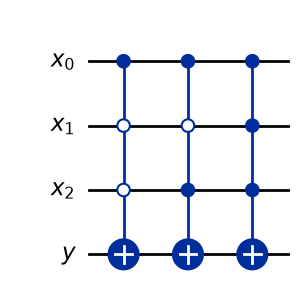
\includegraphics[width=\textwidth]{imagenes/bloque1/e1_4_oraculo3bits.png}
        \caption{Con \texttt{ctrl\_state}.}
    \end{subfigure}
    \hfill
    \begin{subfigure}{0.65\textwidth}
        \centering
        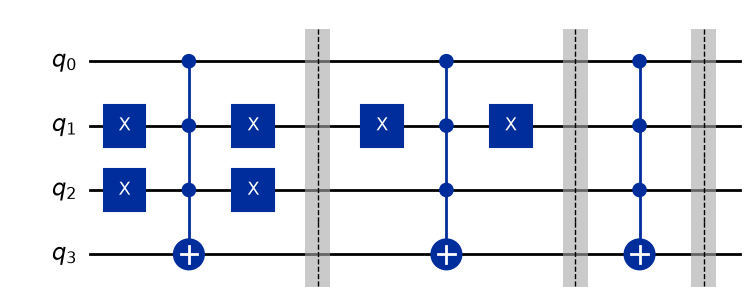
\includegraphics[width=\textwidth]{imagenes/bloque1/e1_4_oraculo3bit_impl.png}
        \caption{Con puertas $X$ explícitas.}
    \end{subfigure}
    \caption{Oráculo de 3 bits del ejercicio 1.4.}\label{fig:bloque1_e1_4_oraculos}
\end{figure}

Para comprobar el oráculo se prepara cada una de las ocho entradas con puertas $X$, se aplica $U_f$ y se miden los cuatro qubits (cadena \texttt{y x2 x1 x0}).
La Figura~\ref{fig:bloque1_e1_4_prueba} muestra, como ejemplo, el circuito de prueba para la entrada $x_2x_1x_0=101$, y la Tabla~\ref{tab:bloque1_e1_4} recoge el resultado para las ocho entradas.

\begin{figure}[h]
    \centering
    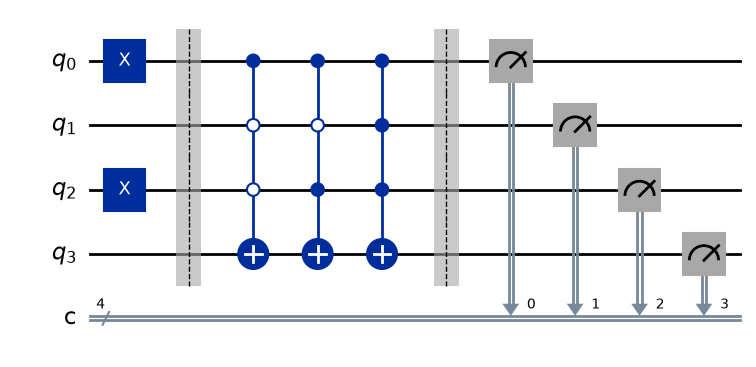
\includegraphics[width=0.6\textwidth]{imagenes/bloque1/e1_4_circuito_prueba.png}
    \caption{Circuito de prueba para la entrada $x_2x_1x_0=101$.}\label{fig:bloque1_e1_4_prueba}
\end{figure}

\begin{table}[htbp]
    \centering
\begin{tabular}{c|c|c|c|c}
\hline
$x_2x_1x_0$ & $f(x)$ teórica & $f(x)$ simulada & $x$ tras $U_f$ & Prob. \\
\hline
\texttt{000} & \texttt{0} & \texttt{0} & \texttt{000} & 1 \\
\texttt{001} & \texttt{1} & \texttt{1} & \texttt{001} & 1 \\
\texttt{010} & \texttt{0} & \texttt{0} & \texttt{010} & 1 \\
\texttt{011} & \texttt{0} & \texttt{0} & \texttt{011} & 1 \\
\texttt{100} & \texttt{0} & \texttt{0} & \texttt{100} & 1 \\
\texttt{101} & \texttt{1} & \texttt{1} & \texttt{101} & 1 \\
\texttt{110} & \texttt{0} & \texttt{0} & \texttt{110} & 1 \\
\texttt{111} & \texttt{1} & \texttt{1} & \texttt{111} & 1 \\
\hline
\end{tabular}
    \caption{Ejercicio 1.4: tabla de verdad simulada junto a la teórica.}\label{tab:bloque1_e1_4}
\end{table}

\textbf{Resultado.} Las ocho entradas producen $y=f(x)$ con probabilidad 1 y sin alterar $x$: la salida es 1 únicamente para $x_2x_1x_0=001,\,101,\,111$,
tal como indica la tabla del enunciado. Cada minitérmino activa una sola de las tres puertas, porque cada una solo se dispara con su propia entrada; por eso basta con componerlas
(se suman módulo 2 sobre $y$ sin solaparse). El operador coincide con el de la construcción con puertas $X$ explícitas y cumple $U_f^2=I$.

%--------------------------------------------------------------------
\subsection{Ejercicio 1.5. Oráculo de 4 bits de entrada y 4 de salida}
La tabla de la función se codifica en un diccionario de Python \texttt{\{`x3x2x1x0': `f3f2f1f0'\}} y el circuito se genera automáticamente recorriendo sus filas:
por cada fila y por cada bit $f_j=1$ se añade una \texttt{MCXGate(4)} con controles en $q_0\dots q_3$ (con \texttt{ctrl\_state} igual al propio $x$) y objetivo en $q_{4+j}$.
Las entradas están en $q_0\dots q_3$ y las salidas en $q_4\dots q_7$, siguiendo la cabecera de la tabla: $f_0\to q_4$ y $f_3\to q_7$.

\textbf{Predicción.} El número de puertas multicontroladas debe ser igual al número total de unos de la tabla, que es 32, y la cadena medida es \texttt{f3 f2 f1 f0 x3 x2 x1 x0}.
En el circuito generado (Figura~\ref{fig:bloque1_e1_5_oraculo}) se obtienen, en efecto, 32 puertas.

\begin{figure}[h]
    \centering
    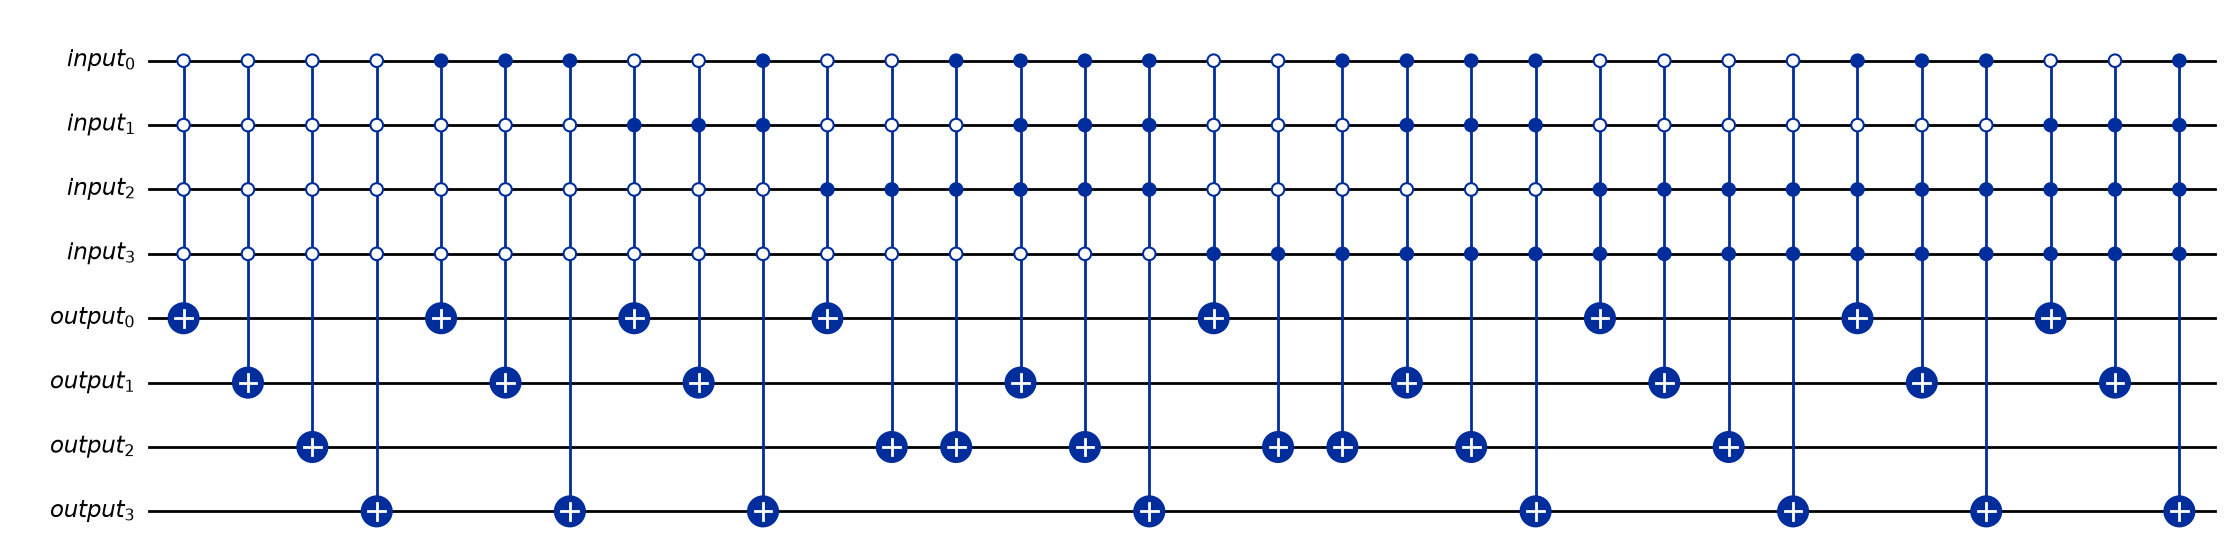
\includegraphics[width=\textwidth]{imagenes/bloque1/e1_5_oraculos4bits.png}
    \caption{Oráculo del ejercicio 1.5 (32 puertas multicontroladas).}\label{fig:bloque1_e1_5_oraculo}
\end{figure}

\begin{table}[htbp]
    \centering
{\small\setlength{\tabcolsep}{4pt}
\begin{tabular}{c|c|c|c||c|c|c|c}
\hline
$x_3x_2x_1x_0$ & teórica & simulada & Prob. & $x_3x_2x_1x_0$ & teórica & simulada & Prob. \\
\hline
\texttt{0000} & \texttt{1111} & \texttt{1111} & 1 & \texttt{1000} & \texttt{0101} & \texttt{0101} & 1 \\
\texttt{0001} & \texttt{1011} & \texttt{1011} & 1 & \texttt{1001} & \texttt{0100} & \texttt{0100} & 1 \\
\texttt{0010} & \texttt{0011} & \texttt{0011} & 1 & \texttt{1010} & \texttt{0000} & \texttt{0000} & 1 \\
\texttt{0011} & \texttt{1000} & \texttt{1000} & 1 & \texttt{1011} & \texttt{1110} & \texttt{1110} & 1 \\
\texttt{0100} & \texttt{0101} & \texttt{0101} & 1 & \texttt{1100} & \texttt{1111} & \texttt{1111} & 1 \\
\texttt{0101} & \texttt{0100} & \texttt{0100} & 1 & \texttt{1101} & \texttt{1011} & \texttt{1011} & 1 \\
\texttt{0110} & \texttt{0000} & \texttt{0000} & 1 & \texttt{1110} & \texttt{0011} & \texttt{0011} & 1 \\
\texttt{0111} & \texttt{1110} & \texttt{1110} & 1 & \texttt{1111} & \texttt{1000} & \texttt{1000} & 1 \\
\hline
\end{tabular}}
    \caption{Ejercicio 1.5: $f_3f_2f_1f_0$ teórica y simulada para las 16 entradas, con la probabilidad (frecuencia sobre 4096 disparos) con la que se obtiene
    cada resultado. En los 16 casos la entrada se mide intacta tras $U_f$.}\label{tab:bloque1_e1_5}
\end{table}

\textbf{Resultado.} Las 16 entradas dan la salida de la tabla con probabilidad 1 y las entradas quedan intactas (Tabla~\ref{tab:bloque1_e1_5}).
Esta función $f:\{0,1\}^4\to\{0,1\}^4$ no es inyectiva (hay salidas repetidas, como \texttt{0101} o \texttt{1111}), por lo que por sí sola no sería reversible. Sin embargo, el oráculo $U_f$
es siempre unitario e involutivo, gracias a que la entrada se conserva y la salida se suma módulo 2: su matriz es una permutación de la base computacional
de 8 qubits y cumple $U_f^2=I$, como se ha comprobado numéricamente.



%--------------------------------------------------------------------
\subsection{Ejercicio 1.6. Función lineal $f(x) = a\cdot x$}
Para $a=a_4a_3a_2a_1a_0=11010$ se tiene $f(x)=a\cdot x=x_4\oplus x_3\oplus x_1$. Una función lineal no necesita puertas multicontroladas:
basta un CNOT desde cada qubit $q_i\equiv x_i$ con $a_i=1$ hacia la ancilla $q_5\equiv y$. En este caso son tres CNOT, desde $q_4$, $q_3$ y $q_1$
(Figura~\ref{fig:bloque1_e1_6_oraculo}).

\begin{figure}[h]
    \centering
    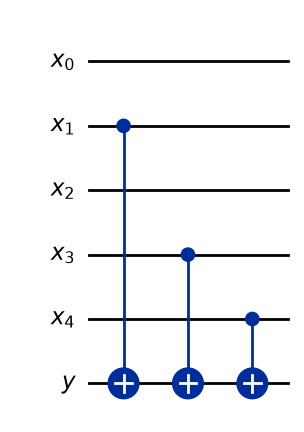
\includegraphics[width=0.3\textwidth]{imagenes/bloque1/e1_6_oraculosBV.png}
    \caption{Oráculo lineal $f(x)=x_4\oplus x_3\oplus x_1$.}\label{fig:bloque1_e1_6_oraculo}
\end{figure}

\textbf{Predicción.} $y=1$ exactamente en las entradas con un número impar de unos entre $x_4,x_3,x_1$ (16 de las 32), y la cadena medida es \texttt{y x4 x3 x2 x1 x0}.

\begin{table}[htbp]
    \centering
{\small\setlength{\tabcolsep}{4pt}
\begin{tabular}{c|c|c|c||c|c|c|c}
\hline
$x_4x_3x_2x_1x_0$ & teórica & simulada & Prob. & $x_4x_3x_2x_1x_0$ & teórica & simulada & Prob. \\
\hline
\texttt{00000} & \texttt{0} & \texttt{0} & 1 & \texttt{10000} & \texttt{1} & \texttt{1} & 1 \\
\texttt{00001} & \texttt{0} & \texttt{0} & 1 & \texttt{10001} & \texttt{1} & \texttt{1} & 1 \\
\texttt{00010} & \texttt{1} & \texttt{1} & 1 & \texttt{10010} & \texttt{0} & \texttt{0} & 1 \\
\texttt{00011} & \texttt{1} & \texttt{1} & 1 & \texttt{10011} & \texttt{0} & \texttt{0} & 1 \\
\texttt{00100} & \texttt{0} & \texttt{0} & 1 & \texttt{10100} & \texttt{1} & \texttt{1} & 1 \\
\texttt{00101} & \texttt{0} & \texttt{0} & 1 & \texttt{10101} & \texttt{1} & \texttt{1} & 1 \\
\texttt{00110} & \texttt{1} & \texttt{1} & 1 & \texttt{10110} & \texttt{0} & \texttt{0} & 1 \\
\texttt{00111} & \texttt{1} & \texttt{1} & 1 & \texttt{10111} & \texttt{0} & \texttt{0} & 1 \\
\texttt{01000} & \texttt{1} & \texttt{1} & 1 & \texttt{11000} & \texttt{0} & \texttt{0} & 1 \\
\texttt{01001} & \texttt{1} & \texttt{1} & 1 & \texttt{11001} & \texttt{0} & \texttt{0} & 1 \\
\texttt{01010} & \texttt{0} & \texttt{0} & 1 & \texttt{11010} & \texttt{1} & \texttt{1} & 1 \\
\texttt{01011} & \texttt{0} & \texttt{0} & 1 & \texttt{11011} & \texttt{1} & \texttt{1} & 1 \\
\texttt{01100} & \texttt{1} & \texttt{1} & 1 & \texttt{11100} & \texttt{0} & \texttt{0} & 1 \\
\texttt{01101} & \texttt{1} & \texttt{1} & 1 & \texttt{11101} & \texttt{0} & \texttt{0} & 1 \\
\texttt{01110} & \texttt{0} & \texttt{0} & 1 & \texttt{11110} & \texttt{1} & \texttt{1} & 1 \\
\texttt{01111} & \texttt{0} & \texttt{0} & 1 & \texttt{11111} & \texttt{1} & \texttt{1} & 1 \\
\hline
\end{tabular}}
    \caption{Ejercicio 1.6: $f(x)=x_4\oplus x_3\oplus x_1$ para las 32 entradas, con el valor teórico, el simulado y la probabilidad con la que se obtiene
    (frecuencia sobre 4096 disparos). En los 32 casos la entrada se mide intacta tras $U_f$.}\label{tab:bloque1_e1_6}
\end{table}

\textbf{Resultado.} Las 32 entradas coinciden con $f(x)=x_4\oplus x_3\oplus x_1$ (paridad de los bits de $x$ en las posiciones donde $a$ vale 1) con probabilidad 1,
y $x$ no se modifica (Tabla~\ref{tab:bloque1_e1_6}). El oráculo usa solo 3 CNOT, frente a las 16 puertas multicontroladas que requeriría la construcción por minitérminos
para esta función (16 entradas con $f=1$). Este mismo oráculo se reutiliza en el algoritmo de Bernstein-Vazirani (ejercicio 3.3), donde la cadena oculta $a$ se recupera con una única consulta.
\section{Bloque 2}
\label{sec:bloque_2}
\section{Bloque 3. Algoritmos de consulta: Deutsch, Deutsch-Jozsa y Bernstein-Vazirani}\label{sec:bloque_3}

\subsection{Ejercicio 3.1: Algoritmo de Deutsch}
En el siguiente ejercicio se implementa el Algoritmo de Deutsch para cada uno de los casos de funciones binarias de una variable.

\textbf{Oráculo a.} Oráculo de la función constante 0, $f(x) = 0$. Es una función constante, por lo tanto tras ejecutar el algoritmo
de Deutsch se debería de medir en el qubit de dato $q_0$ el estado $\ket{0}$. En la Figura~\ref{fig:bloque3_e3_1_a} se observa el circuito del algoritmo
y el histograma de la medida sobre el qubit de dato $q_0$. La simulación coincide con la predicción. 

\begin{figure}[h]
    \centering
    \begin{subfigure}{0.48\textwidth}
        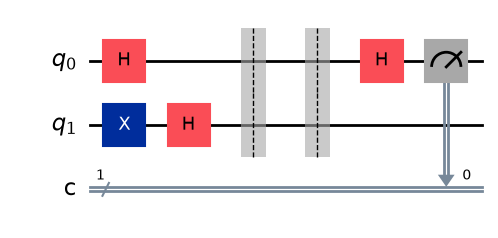
\includegraphics[width=\textwidth]{imagenes/bloque3/e3_1_circuito_a.png}
        \caption{}
    \end{subfigure}
    \hfill
    \begin{subfigure}{0.48\textwidth}
        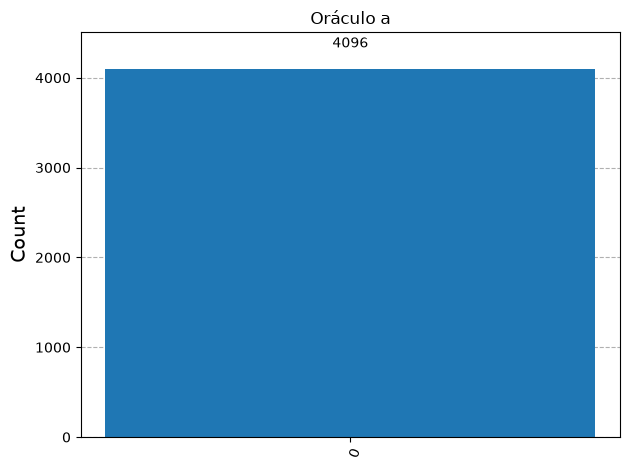
\includegraphics[width=0.7\textwidth]{imagenes/bloque3/e3_1_histograma_a.png}
        \caption{}
    \end{subfigure}
    \caption{(a): Circuito construido para Oráculo a. \\
    (b): Histograma del algoritmo de Deutsch para el Oráculo a.}\label{fig:bloque3_e3_1_a}
\end{figure}


\textbf{Oráculo b.} Oráculo de la función constante 1, $f(x) = 1$. Es una función constante, por lo tanto tras ejecutar el algoritmo
de Deutsch se debería de medir en el qubit de dato $q_0$ el estado $\ket{0}$. En la Figura~\ref{fig:bloque3_e3_1_b} se observa el circuito del algoritmo
y el histograma de la medida sobre el qubit de dato $q_0$. La simulación coincide con la predicción. 

\begin{figure}[h]
    \centering
    \begin{subfigure}{0.48\textwidth}
        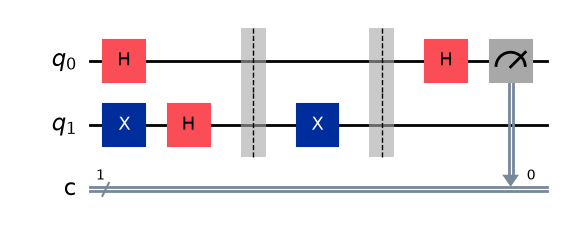
\includegraphics[width=\textwidth]{imagenes/bloque3/e3_1_circuito_b.png}
        \caption{}
    \end{subfigure}
    \hfill
    \begin{subfigure}{0.48\textwidth}
        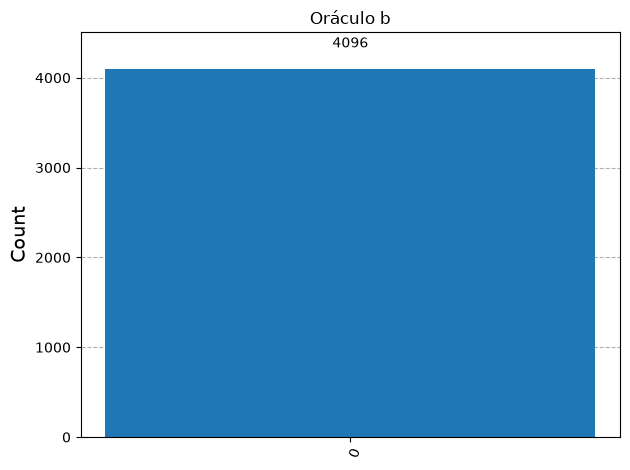
\includegraphics[width=0.7\textwidth]{imagenes/bloque3/e3_1_histograma_b.png}
        \caption{}
    \end{subfigure}
    \caption{(a): Circuito construido para Oráculo b. \\
    (b): Histograma del algoritmo de Deutsch para el Oráculo b.}\label{fig:bloque3_e3_1_b}
\end{figure}

\textbf{Oráculo c.} Oráculo de la función identidad $f(x) = x$. Es una función balanceada, por lo tanto tras ejecutar el algoritmo
de Deutsch se debería de medir en el qubit de dato $q_0$ el estado $\ket{1}$. En la Figura~\ref{fig:bloque3_e3_1_c} se observa el circuito del algoritmo
y el histograma de la medida sobre el qubit de dato $q_0$. La simulación coincide con la predicción. 
\begin{figure}[h]
    \centering
    \begin{subfigure}{0.48\textwidth}
        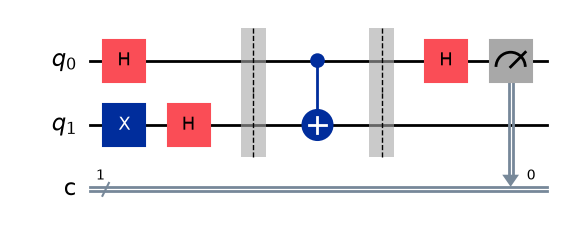
\includegraphics[width=\textwidth]{imagenes/bloque3/e3_1_circuito_c.png}
        \caption{}
    \end{subfigure}
    \hfill
    \begin{subfigure}{0.48\textwidth}
        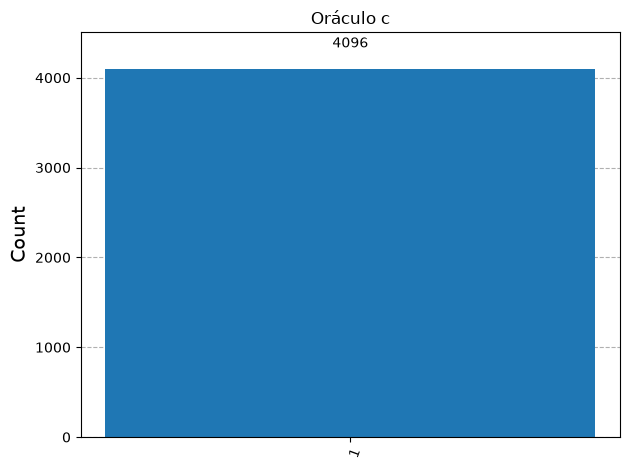
\includegraphics[width=0.7\textwidth]{imagenes/bloque3/e3_1_histograma_c.png}
        \caption{}
    \end{subfigure}
    \caption{(a): Circuito construido para Oráculo c. \\
    (b): Histograma del algoritmo de Deutsch para el Oráculo c.}\label{fig:bloque3_e3_1_c}
\end{figure}

\textbf{Oráculo d.} Oráculo de la función inversa, $f(x) = NOT(x)$. Es una función balanceada, por lo tanto tras ejecutar el algoritmo
de Deutsch se debería de medir en el qubit de dato $q_0$ el estado $\ket{1}$. En la Figura~\ref{fig:bloque3_e3_1_d} se observa el circuito del algoritmo
y el histograma de la medida sobre el qubit de dato $q_0$. La simulación coincide con la predicción. 

\begin{figure}[h]
    \centering
    \begin{subfigure}{0.48\textwidth}
        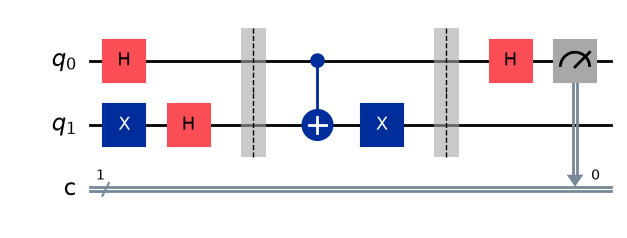
\includegraphics[width=\textwidth]{imagenes/bloque3/e3_1_circuito_d.png}
        \caption{}
    \end{subfigure}
    \hfill
    \begin{subfigure}{0.48\textwidth}
        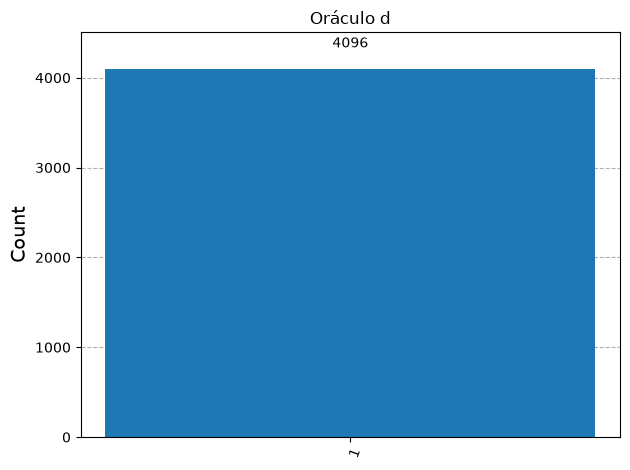
\includegraphics[width=0.7\textwidth]{imagenes/bloque3/e3_1_histograma_d.png}
        \caption{}
    \end{subfigure}
    \caption{(a): Circuito construido para Oráculo d. \\
    (b): Histograma del algoritmo de Deutsch para el Oráculo d.}\label{fig:bloque3_e3_1_d}
\end{figure}


\subsection{Ejercicio 3.2: Deutsch-Jozsa con \texorpdfstring{$n=2$}{n=2}}
En el siguiente ejercicio se implementa el algoritmo de Deutsch-Jozsa para una serie de funciones y se evalúa los histogramas de la simulación.

\textbf{Función a.} Función constante 0, $f(x_1, x_0) = 0$. En la Figura~\ref{fig:bloque3_e3_2_a} se muestra el oráculo para la 
función especificada en este apartado. Al ser una función constante, el valor medido en los qubits de datos tras la ejecución del algoritmo sería
$\ket{00}$ que efectivamente se cumple en el histograma mostrado en la Figura mencionada.

\begin{figure}[]
    \centering
    \begin{subfigure}{0.4\textwidth}
        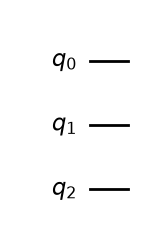
\includegraphics[width=0.4\textwidth]{imagenes/bloque3/e3_2_oraculo_a.png}
        \caption{}
    \end{subfigure}
    %\hfill
    \begin{subfigure}{0.4\textwidth}
        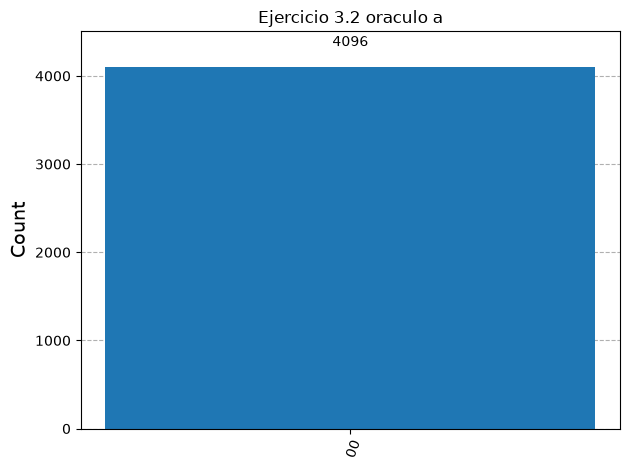
\includegraphics[width=0.75\textwidth]{imagenes/bloque3/e3_2_histograma_a.png}
        \caption{}
    \end{subfigure}
    \caption{(a): Circuito construido para Oráculo a. \\
    (b): Histograma del algoritmo de Deutsch-Jozsa para el Oráculo a.}\label{fig:bloque3_e3_2_a}
\end{figure}

\textbf{Función b.} Función $f(x_1, x_0) = x_1 \oplus x_0$. En la Figura~\ref{fig:bloque3_e3_2_b} se muestra el oráculo implementado
para esta función junto al histograma del resultado de la medida tras la ejecución del algoritmo. El resultado medido corresponde al estado
$\ket{11}$ lo que indica que la función es balanceada.

\begin{figure}[h]
    \centering
    \begin{subfigure}{0.4\textwidth}
        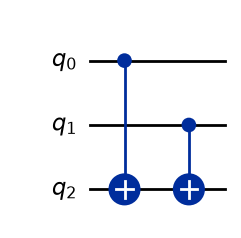
\includegraphics[width=0.5\textwidth]{imagenes/bloque3/e3_2_oraculo_b.png}
        \caption{}
    \end{subfigure}
    %\hfill
    \begin{subfigure}{0.4\textwidth}
        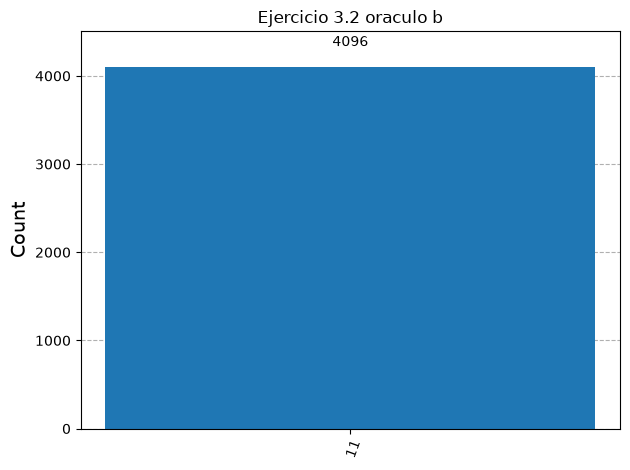
\includegraphics[width=0.75\textwidth]{imagenes/bloque3/e3_2_histograma_b.png}
        \caption{}
    \end{subfigure}
    \caption{(a): Circuito construido para Oráculo b. \\
    (b): Histograma del algoritmo de Deutsch-Jozsa para el Oráculo b.}\label{fig:bloque3_e3_2_b}
\end{figure}

\begin{figure}[h]
    \centering
    \begin{subfigure}{0.4\textwidth}
        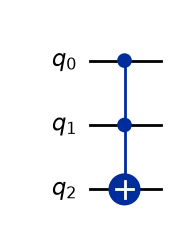
\includegraphics[width=0.45\textwidth]{imagenes/bloque3/e3_2_oraculo_c.png}
        \caption{}
    \end{subfigure}
    %\hfill
    \begin{subfigure}{0.4\textwidth}
        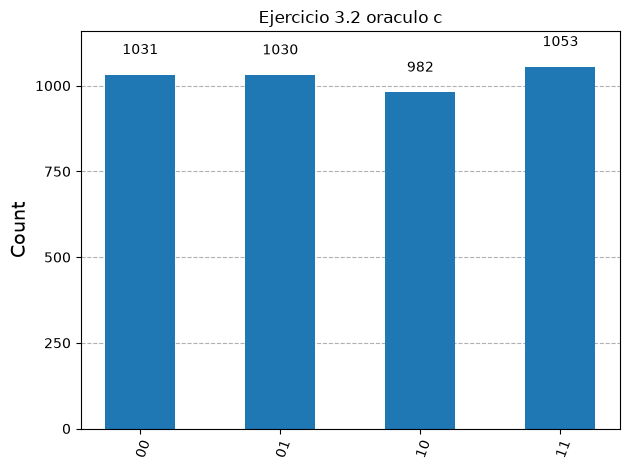
\includegraphics[width=0.75\textwidth]{imagenes/bloque3/e3_2_histograma_c.png}
        \caption{}
    \end{subfigure}
    \caption{(a): Circuito construido para Oráculo c. \\
    (b): Histograma del algoritmo de Deutsch-Jozsa para el Oráculo c.}\label{fig:bloque3_e3_2_c}
\end{figure}

\textbf{Función c.} Función $f(x_1, x_0) = x_1 \land x_0$. En la
Figura~\ref{fig:bloque3_e3_2_c} se muestra el oráculo implementado para
esta función junto al histograma del resultado de la medida tras la
ejecución del algoritmo. El oráculo se implementa con una puerta Toffoli
que suma la operación AND de los dos primeros qubits sobre el último. En
el histograma aparecen las cuatro cadenas, entre ellas $\ket{00}$ y otras
que no lo son.

\textbf{Predicción y por qué no se puede concluir.} Para
$f(x_1,x_0)=x_1\wedge x_0$ solo hay un $1$ entre las cuatro entradas
($f(11)=1$), de modo que $f$ no es constante ni balanceada y no cumple la
promesa de Deutsch-Jozsa. La amplitud de la cadena $z=z_1z_0$ al final
del algoritmo es
\[
  \alpha_z=\frac14\sum_{x_1,x_0}(-1)^{\,f(x_1,x_0)\,\oplus\,(z_1x_1\oplus z_0x_0)},
\]
que da $\alpha_{00}=\alpha_{01}=\alpha_{10}=\tfrac12$ y
$\alpha_{11}=-\tfrac12$ (por ejemplo,
$\alpha_{00}=\tfrac14(1+1+1-1)=\tfrac12$). Por tanto, las cuatro cadenas
se miden con probabilidad $|\alpha_z|^2=1/4$. La simulación lo confirma
(Figura~\ref{fig:bloque3_e3_2_c}b): se obtienen 1031, 1030, 982 y 1053
conteos de 4096 frente a los 1024 esperados ($\chi^2=2{,}63$ con
3 grados de libertad, $p=0{,}453$).

Si $f$ fuese constante se mediría $00$ con probabilidad $1$, y si fuese
balanceada no se mediría nunca ($\alpha_{00}=0$). Aquí $00$ aparece con
probabilidad $1/4$, que no corresponde a ninguno de los dos casos, y el
resto de cadenas tampoco permite distinguirlos. Como la promesa no se
cumple, la medida carece de interpretación y no se puede extraer ninguna
conclusión de ella sobre el tipo de $f$.

\subsection{Ejercicio 3.3: Bernstein-Vazirani}\label{subsection:ejercicio3_3}
En este ejercicio se ha implementado el algoritmo de Bernstein-Vazirani para obtener una clave $a = 1010$, construyendo el oráculo
correspondiente. En la Figura~\ref{fig:bloque3_e3_3_a1} se puede observar el oráculo implementado para dicha clave $a$. También se ha simulado
el algoritmo con un único \textit{shot} y se ha podido conseguir la clave, tal y como se pide en el enunciado.

\textbf{Observación: } A la hora de realizar la medida se ha invertido el orden de los bits clásicos a los que corresponden cada qubit. Es decir, 
al qubit $q_0$ se le ha asignado el bit clásico más significativo en la medida, y $q_3$ (el más significativo) se le ha asignado el bit clásico 
menos significativo. La implementación del oráculo se ha realizado teniendo la notación contraria de qubits a la de Qiskit, por lo que la inversión
del orden nos permite tener la notación correcta en los resultados de medida.
\begin{figure}[h]
    \centering
    \begin{subfigure}{0.4\textwidth}
        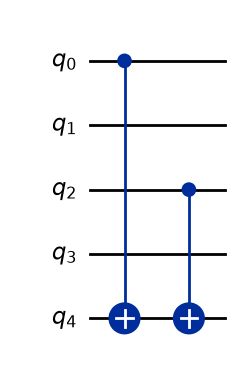
\includegraphics[width=0.5\textwidth]{imagenes/bloque3/e3_3_oraculo_a1.png}
        \caption{}
    \end{subfigure}
    %\hfill
    \begin{subfigure}{0.4\textwidth}
        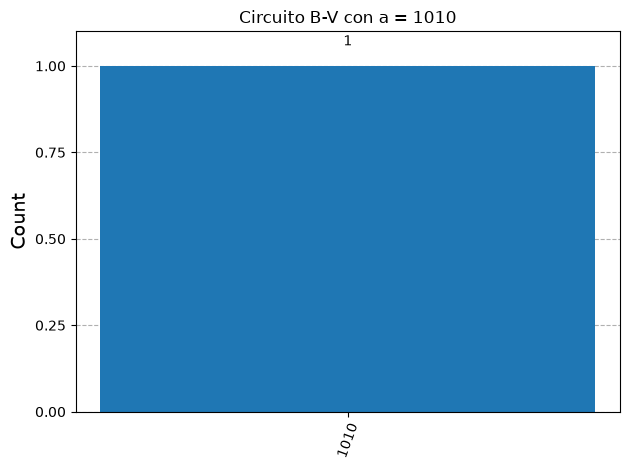
\includegraphics[width=0.8\textwidth]{imagenes/bloque3/e3_3_histograma_a1.png}
        \caption{}
    \end{subfigure}
    \caption{(a): Oráculo para la clave $a = 1010$. \\
    (b): Histograma de la ejecución del algoritmo para obtener la clave $a = 1010$}\label{fig:bloque3_e3_3_a1}
\end{figure}

Por otro lado, como segunda prueba, se ha escogido otra clave $a = 1101$ y se ha implementado el algoritmo. En la Figura~\ref{fig:bloque3_e3_3_a2}
se incluye el oráculo correspondiente junto al histograma de la ejecución con un único shot. Nuevamente se consigue obtener la clave secreta.

\begin{figure}[h]
    \centering
    \begin{subfigure}{0.4\textwidth}
        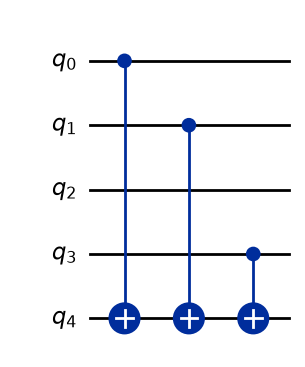
\includegraphics[width=0.5\textwidth]{imagenes/bloque3/e3_3_oraculo_a2.png}
        \caption{}
    \end{subfigure}
    %\hfill
    \begin{subfigure}{0.4\textwidth}
        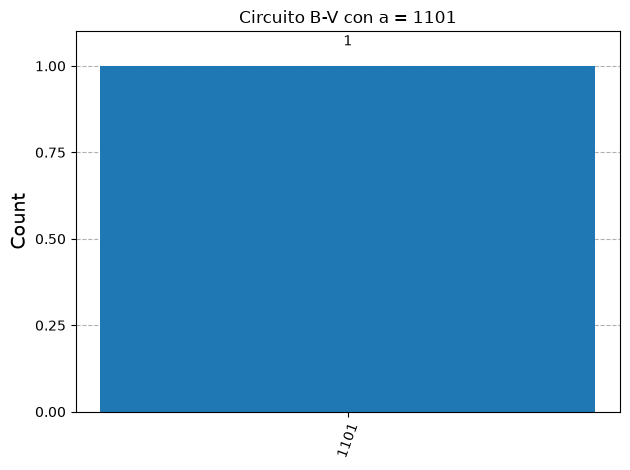
\includegraphics[width=0.8\textwidth]{imagenes/bloque3/e3_3_histograma_a2.png}
        \caption{}
    \end{subfigure}
    \caption{(a): Oráculo para la clave $a = 1101$. \\
    (b): Histograma de la ejecución del algoritmo para obtener la clave $a = 1101$}\label{fig:bloque3_e3_3_a2}
\end{figure}



\subsection{Ejercicio E1: Deutsch-Jozsa con un oráculo dado}
En este ejercicio se implementa el algoritmo de Deutsch-Jozsa para un oráculo dado y se quiere determinar qué tipo de función 
$f(x_0, x_1)$ corresponde (constante o balanceada). En la Figura~\ref{fig:bloque3_e1_algoritmo_df} se muestra el oráculo detallado
en el enunciado y el circuito que implementa el Algoritmo de Deutsch-Jozsa correspondiente.

\begin{figure}[h]
    \centering
    \begin{subfigure}{0.48\textwidth}
        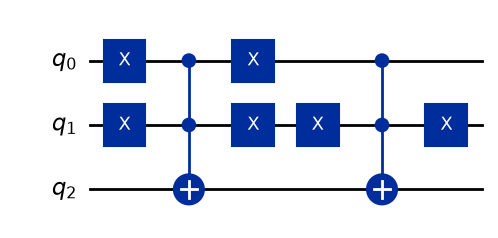
\includegraphics[width=0.9\textwidth]{imagenes/bloque3/e1_oraculo_df.png}
        \caption{}
    \end{subfigure}
    %\hfill
    \begin{subfigure}{0.48\textwidth}
        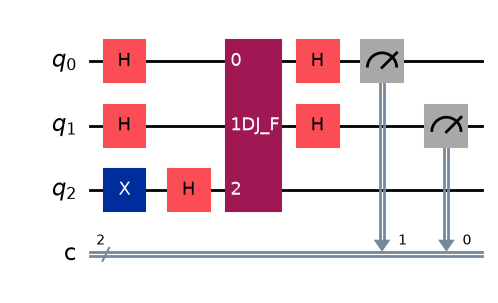
\includegraphics[width=0.9\textwidth]{imagenes/bloque3/e1_circuito.png}
        \caption{}
    \end{subfigure}
    \caption{(a): Oráculo $DJ\_F$ del enunciado. \\
    (b): Circuito que implementa el algoritmo de Deutsch-Jozsa}\label{fig:bloque3_e1_algoritmo_df}
\end{figure}

Tras simular el circuito, se mide el estado $\ket{01}$ que aparece en la Figura~\ref{fig:bloque3_e1_histograma_algoritmo}. Se ha realizado la misma inversión
del orden de los bits clásicos en la medida respecto de los qubits al igual que en el ejercicio anterior. Por lo tanto, el estado medido es $\ket{q_0, q_1} = \ket{01}$.

Con esta medición, de acuerdo a la formulación del algoritmo, se puede deducir que la amplitud del estado $\ket{00}$ es $0$, por lo que se puede
concluir que la función $f$ es \textbf{balanceada}. 
\begin{figure}
    \centering
    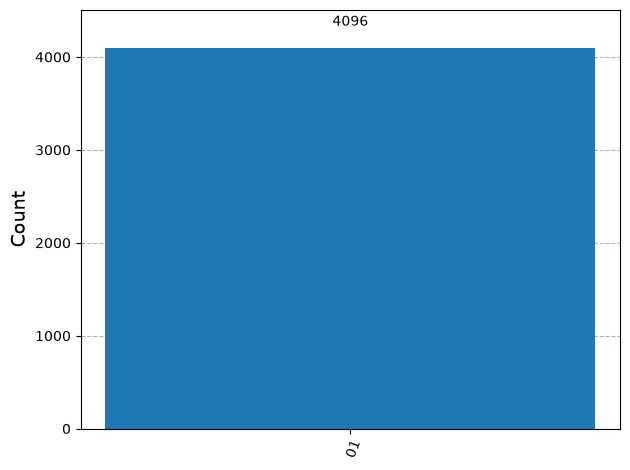
\includegraphics[width=0.35\textwidth]{imagenes/bloque3/e1_histograma_algoritmo.png}
    \caption{Histograma de la ejecución del algoritmo de Deutsch-Jozsa para el oráculo $DJ\_F$}\label{fig:bloque3_e1_histograma_algoritmo}
\end{figure}

Por otro lado, para obtener la tabla de verdad de la función $f$ se ha simulado el oráculo para cada una de las cuatro entradas
de la base computacional de los qubits $q_0, q_1$. Para evaluar la salida para cada entrada se ha inicializado $\ket{q_2} = \ket{0}$.
En la Figura~\ref{fig:bloque3_e1_histogramas} se puede visualizar el valor de las salidas de $f$ para cada una de las $4$ entradas
de la base computacional tras simular por separado el oráculo. Con ello podemos construir la tabla de verdad de $f$ y se deduce 
que la función simplificada es: $f(x_0, x_1) = \overline{x_1}$ (la barra denota que $f$ vale $1$ cuando $x_1 = 0$).
\begin{table}[htbp]
    \centering
    \begin{tabular}{c c c c}
        \toprule
        $x_0$ & $x_1$ & $x$ & $f(x)$ \\
        \midrule
        0 & 0 & 0 & 1 \\
        0 & 1 & 1 & 0 \\
        1 & 0 & 2 & 1 \\
        1 & 1 & 3 & 0 \\
        \bottomrule
    \end{tabular}
    \caption{Tabla de verdad de la función $f$.}\label{tab:bloque3_e1_tablaverdad}
\end{table}

\begin{figure}[htbp]
    \centering
    \begin{subfigure}{0.4\textwidth}
        \centering
        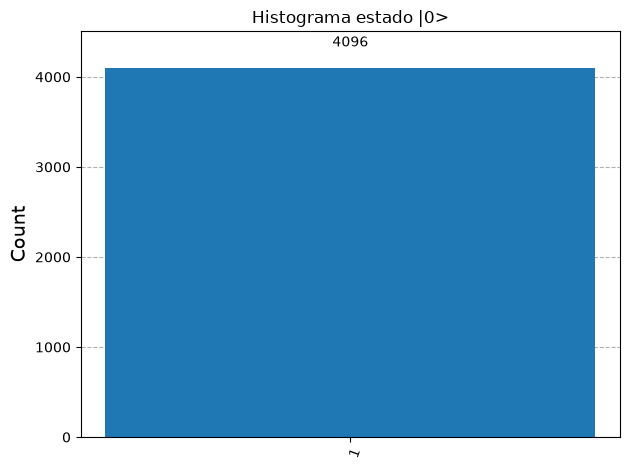
\includegraphics[width=\textwidth]{imagenes/bloque3/e1_histograma_f00.png}
        \caption{}
    \end{subfigure}
    \hfill
    \begin{subfigure}{0.4\textwidth}
        \centering
        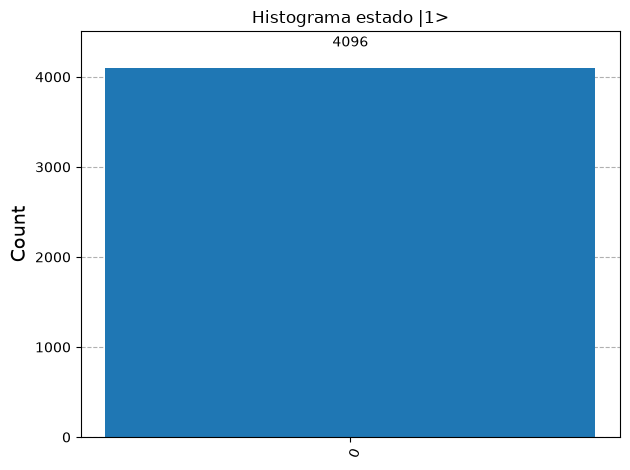
\includegraphics[width=\textwidth]{imagenes/bloque3/e1_histograma_f01.png}
        \caption{}
    \end{subfigure}

    \bigskip
    \begin{subfigure}{0.4\textwidth}
        \centering
        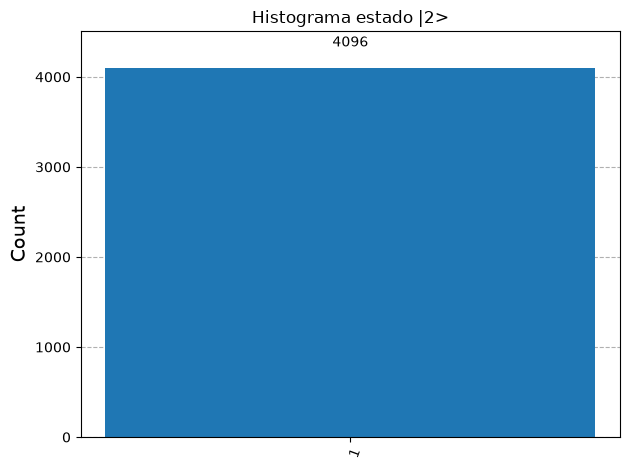
\includegraphics[width=\textwidth]{imagenes/bloque3/e1_histograma_f10.png}
        \caption{}
    \end{subfigure}
    \hfill
    \begin{subfigure}{0.4\textwidth}
        \centering
        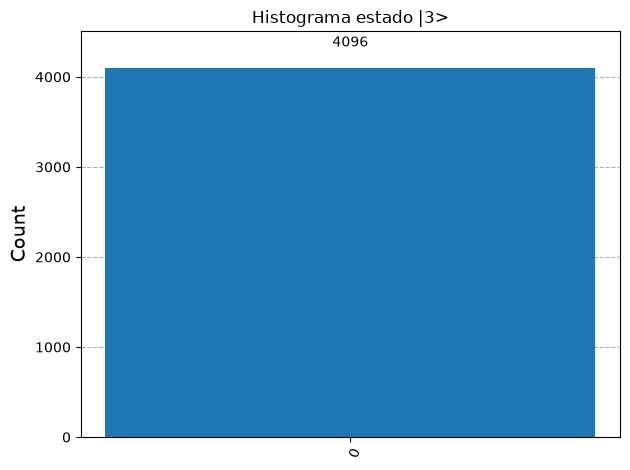
\includegraphics[width=\textwidth]{imagenes/bloque3/e1_histograma_f11.png}
        \caption{}
    \end{subfigure}
    \caption{Resultados de medición sobre $q_2$ tras simular el oráculo $DJ\_F$ para cada uno de las 
    $4$ entradas de la base computacional: $\ket{00}, \ket{01}, \ket{10}$ y $\ket{11}$}\label{fig:bloque3_e1_histogramas}
\end{figure}


El algoritmo de Bernstein--Vazirani trata funciones de la forma
$f(x)=s\cdot x\oplus b$, con $s\in\{0,1\}^n$, $s\cdot x=s_0x_0\oplus s_1x_1$ y
$b\in\{0,1\}$. Se usa el orden $(x_0,x_1)$, con el bit de $q_0$ primero. Del apartado (d),
\[
  f(x_0,x_1)=\overline{x_1}=x_1\oplus 1
  \quad\Longrightarrow\quad s=(s_0,s_1)=(0,1),\qquad b=1 .
\]
Con el auxiliar en $\ket{-}$, el or\'aculo act\'ua por \emph{phase kickback} y, antes de la
$H$ final, el registro de consulta queda en
\[
  \frac{1}{2}\sum_{x}(-1)^{f(x)}\ket{x}
  =(-1)^{b}\,\frac{1}{2}\sum_{x}(-1)^{s\cdot x}\ket{x}
  =(-1)^{b}\,H^{\otimes 2}\ket{s}.
\]
Al aplicar la $H$ final y usar $H^{\otimes 2}H^{\otimes 2}=\mathbb{I}$, el registro queda en
$(-1)^{b}\ket{s}$. De forma equivalente, la amplitud de cada cadena $z$ es
\[
  \alpha_z=\frac{1}{4}\sum_{x}(-1)^{f(x)\oplus z\cdot x}
  =\frac{(-1)^{b}}{4}\sum_{x}(-1)^{(s\oplus z)\cdot x}
  =(-1)^{b}\,\delta_{z,s},
\]
por la ortogonalidad de los caracteres $(-1)^{w\cdot x}$ (la suma vale $4$ si $z=s$ y $0$
en caso contrario). Por tanto:
\begin{itemize}
  \item se mide $z=s$ con probabilidad $|\alpha_s|^2=1$, de modo que la cadena medida en el apartado (b),
        $(c_0,c_1)=(0,1)$, es exactamente el vector $s$ de la f\'ormula obtenida en el apartado(d):
        $s_1=1$ indica que $f$ depende de $x_1$, y $s_0=0$ que no depende de $x_0$;
  \item el t\'ermino $b$ solo aporta una fase global $(-1)^b$ y no se observa en la medici\'on;
  \item el algoritmo devuelve una \'unica cadena porque $f$ es \emph{af\'in}: toda la amplitud
        se concentra en $z=s$. Si $f$ no fuera af\'in, la amplitud se repartir\'ia entre
        varias cadenas;
  \item como $s\neq 00$, se confirma que $f$ es balanceada, de acuerdo con el apartado (c).
\end{itemize}





\section{Bloque 4}\label{sec:bloque_4}

\textbf{Convenios del bloque.} El estado marcado se escribe $w=x_{n-1}\dots x_0$, con $x_j$ en el qubit $q_j$ (convenio \emph{little-endian} de Qiskit), de modo que $|w\rangle$
es el elemento de índice $\mathrm{int}(w,2)$ del vector de estado. Para $n=3$ y $w=011$ se marca el estado $|3\rangle$.

El \textbf{oráculo de fase} $O|x\rangle=-|x\rangle$ si $x=w$ y $O|x\rangle=|x\rangle$ en otro caso se construye con una puerta $Z$ multicontrolada
($H\cdot\mathrm{MCX}\cdot H$ sobre el último qubit), rodeando con puertas $X$ los qubits en los que $w$ tiene un 0. El \textbf{operador de difusión}
$D=2|s\rangle\langle s|-I=H^{\otimes n}(2|0\rangle\langle0|-I)H^{\otimes n}$ se implementa con $H^{\otimes n}$, $X^{\otimes n}$, una $Z$ multicontrolada, de nuevo $X^{\otimes n}$ y $H^{\otimes n}$.
Este circuito produce en realidad $-D$ (la $Z$ multicontrolada es $I-2|1\dots1\rangle\langle1\dots1|$, y conjugada con $X^{\otimes n}$ y $H^{\otimes n}$ da $I-2|s\rangle\langle s|$), de modo que se le añade una fase global $\pi$ para que
coincida exactamente con $D$. El algoritmo completo aplica $H^{\otimes n}$ a $|0\rangle^{\otimes n}$, $k$ iteraciones de $G=D\cdot O$ y mide los $n$ qubits.

Para las predicciones se usa $P_k(w)=\sin^2((2k+1)\theta)$ con $\sin\theta=1/\sqrt{N}$. Se emplea \texttt{Statevector} (circuito sin medidas) para las amplitudes y
\texttt{AerSimulator} con 4096 disparos y semilla fija para los histogramas.

%--------------------------------------------------------------------
\subsection{Ejercicio 4.1. Aplicación del operador de difusión}
Para $n=3$ ($N=8$) se parte del estado que resulta de aplicar el oráculo que marca $|3\rangle=|011\rangle$ a la superposición uniforme $|s\rangle=H^{\otimes3}|000\rangle$,
$$|a\rangle=O|s\rangle=\sum_i a_i|i\rangle,\qquad a_i=\tfrac{1}{\sqrt8}\ \ (i\neq3),\qquad a_3=-\tfrac{1}{\sqrt8}.$$
El oráculo de fase correspondiente se muestra en la Figura~\ref{fig:bloque4_e4_1_oraculo}. Como $w=011$ solo tiene un 0 (en el bit de $q_2$), basta una puerta $X$ en $q_2$ antes y después de la $Z$ multicontrolada, que se construye como $H\cdot\mathrm{MCX}\cdot H$ sobre $q_2$.

\begin{figure}[h]
    \centering
    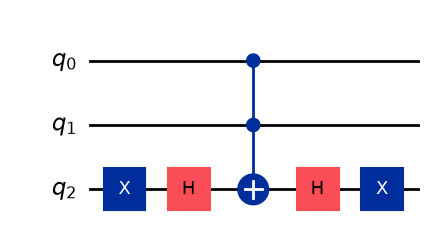
\includegraphics[width=0.6\textwidth]{imagenes/bloque4/e4_1_oraculo.png}
    \caption{Oráculo de fase $O_w$ que marca el estado $|3\rangle=|011\rangle$: $X$ en $q_2$, $Z$ multicontrolada ($H\cdot\mathrm{MCX}\cdot H$ sobre $q_2$) y de nuevo $X$ en $q_2$.}\label{fig:bloque4_e4_1_oraculo}
\end{figure}

\textbf{Cálculo a mano.} La difusión es una inversión respecto a la media, $b_i=2\bar a-a_i$. La media es
$$\bar a=\frac18\Big(7\cdot\frac{1}{\sqrt8}-\frac{1}{\sqrt8}\Big)=\frac{6}{8\sqrt8}=\frac{3}{4\sqrt8}\approx0{,}26517,$$
y por tanto
$$b_i=\frac{3}{2\sqrt8}-\frac{1}{\sqrt8}=\frac{1}{2\sqrt8}\approx0{,}17678\quad(i\neq3),\qquad
b_3=\frac{3}{2\sqrt8}+\frac{1}{\sqrt8}=\frac{5}{2\sqrt8}\approx0{,}88388.$$
La probabilidad de medir el estado marcado pasa de $a_3^2=1/8=0{,}125$ a $b_3^2=25/32\approx0{,}781$. Se comprueba que la suma de probabilidades es 1:
$7\cdot\frac{1}{32}+\frac{25}{32}=1$.

\textbf{Comprobación con el circuito.} El operador de difusión $D=2|s\rangle\langle s|-I=H^{\otimes n}(2|0\rangle\langle0|-I)H^{\otimes n}$ se implementa con el circuito de la Figura~\ref{fig:bloque4_e4_1_difusion}: $H^{\otimes3}$, $X^{\otimes3}$, $Z$ multicontrolada, $X^{\otimes3}$ y $H^{\otimes3}$. Este montaje produce en realidad $-D$, por lo que se le añade una fase global $\pi$ para que coincida exactamente con $D$.

\begin{figure}[h]
    \centering
    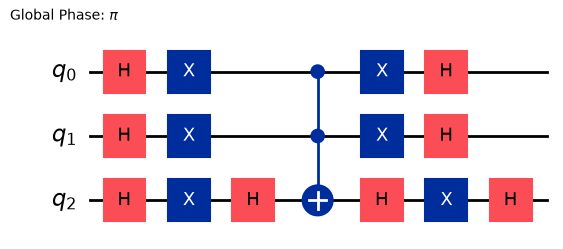
\includegraphics[width=0.6\textwidth]{imagenes/bloque4/e4_1_operado_difusion.png}
    \caption{Circuito del operador de difusión $D$ para $n=3$ (con fase global $\pi$).}\label{fig:bloque4_e4_1_difusion}
\end{figure}

Se verifica con \texttt{Statevector} que: (i) $O|s\rangle=|a\rangle$, (ii) la matriz del circuito
coincide con $2|s\rangle\langle s|-I$ y (iii) $D|a\rangle$ coincide con el vector $|b\rangle$ calculado a mano (Tabla~\ref{tab:bloque4_e4_1}).

\begin{table}[htbp]
    \centering
    \begin{tabular}{c|c|c|c|c}
    \hline
    $i$ & $|i\rangle$ & $a_i$ & $b_i$ (a mano) & $b_i$ (circuito) \\
    \hline
    0 & \texttt{000} &  0,35355 & 0,17678 & 0,17678 \\
    1 & \texttt{001} &  0,35355 & 0,17678 & 0,17678 \\
    2 & \texttt{010} &  0,35355 & 0,17678 & 0,17678 \\
    3 & \texttt{011} & $-0{,}35355$ & 0,88388 & 0,88388 \\
    4 & \texttt{100} &  0,35355 & 0,17678 & 0,17678 \\
    5 & \texttt{101} &  0,35355 & 0,17678 & 0,17678 \\
    6 & \texttt{110} &  0,35355 & 0,17678 & 0,17678 \\
    7 & \texttt{111} &  0,35355 & 0,17678 & 0,17678 \\
    \hline
    \end{tabular}
    \caption{Ejercicio 4.1: amplitudes antes ($a_i$) y después ($b_i$) de aplicar el operador de difusión.}\label{tab:bloque4_e4_1}
\end{table}

El circuito completo de una iteración, $H^{\otimes3}\to O\to D$, se muestra en la Figura~\ref{fig:bloque4_e4_1_completo}; su vector de estado final coincide con $|b\rangle$. La Figura~\ref{fig:bloque4_e4_1_efecto} muestra el efecto de la inversión respecto a la media.

\begin{figure}[h]
    \centering
    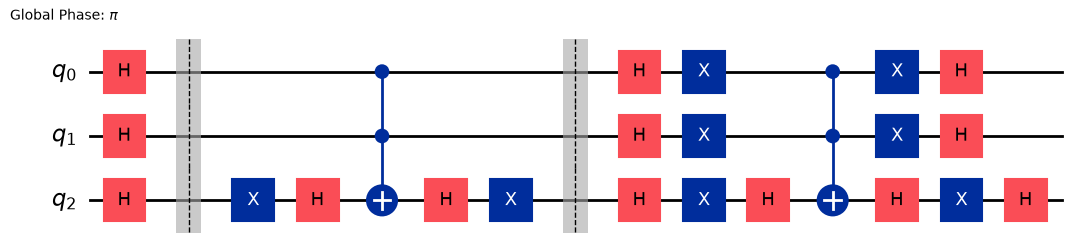
\includegraphics[width=\textwidth]{imagenes/bloque4/e4_1_circuito_completo.png}
    \caption{Circuito completo de una iteración de Grover para $N=8$ y $w=011$: preparación de $|s\rangle$, oráculo $O$ y operador de difusión $D$ (con fase global $\pi$).}\label{fig:bloque4_e4_1_completo}
\end{figure}

\begin{figure}[h]
    \centering
    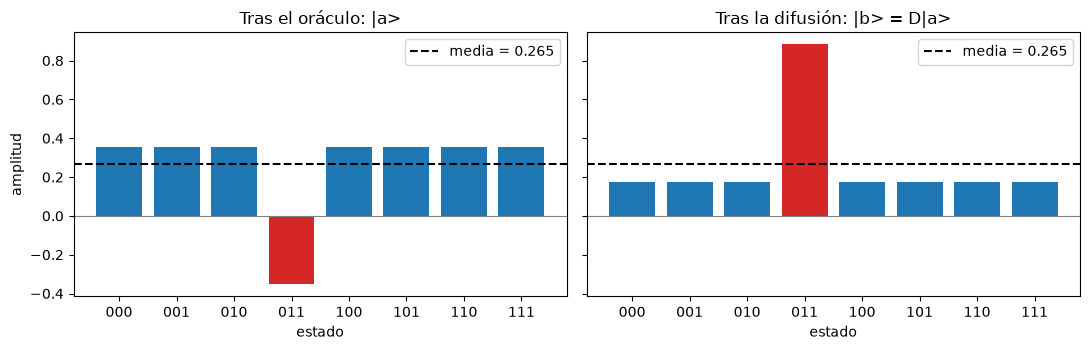
\includegraphics[width=\textwidth]{imagenes/bloque4/e4_1_efecto_difusion.png}
    \caption{Amplitudes tras el oráculo (izquierda) y tras el operador de difusión (derecha). La línea discontinua es la media de las amplitudes; el estado marcado, $|011\rangle$, está en rojo.}\label{fig:bloque4_e4_1_efecto}
\end{figure}

\textbf{Resultado.} El resultado simulado coincide con el calculado a mano. Tras el oráculo, la amplitud del estado marcado es negativa y queda muy por debajo de la media ($0{,}265$);
al invertir respecto a la media pasa de $-0{,}354$ a $+0{,}884$, mientras que las demás amplitudes disminuyen ligeramente, de $0{,}354$ a $0{,}177$. Así, una sola iteración aumenta la probabilidad del estado marcado de $0{,}125$ a $0{,}781$.

%--------------------------------------------------------------------
\subsection{Ejercicio 4.2. Número de iteraciones}
Para $N=8$ y un único estado marcado ($w=011$), $\theta=\arcsin(1/\sqrt8)=0{,}36137$ rad $=20{,}70^\circ$, y la probabilidad de éxito tras $k$ iteraciones es $P_k(w)=\sin^2((2k+1)\theta)$.
La Tabla~\ref{tab:bloque4_e4_2_pk} compara este valor con el obtenido en la simulación para $k=0,\dots,4$.

\begin{table}[htbp]
    \centering
    \begin{tabular}{c|c|c|c}
    \hline
    $k$ & $(2k+1)\theta$ (rad) & $P_k$ teórica & $P_k$ simulada \\
    \hline
    0 & 0,3614 & 0,1250 & 0,1313 \\
    1 & 1,0841 & 0,7813 & 0,7795 \\
    2 & 1,8068 & 0,9453 & 0,9475 \\
    3 & 2,5296 & 0,3301 & 0,3318 \\
    4 & 3,2523 & 0,0122 & 0,0115 \\
    \hline
    \end{tabular}
    \caption{Ejercicio 4.2: probabilidad de éxito de Grover para $N=8$ en función del número de iteraciones $k$.}\label{tab:bloque4_e4_2_pk}
\end{table}

El mínimo número de iteraciones que garantiza al menos un $90\%$ de probabilidad de éxito es $\boldsymbol{k=2}$, con $P_2=0{,}9453$, que concuerda con la estimación $k\approx(\pi/4)\sqrt{N}=2{,}22$.
Con $k=1$ solo se alcanza el $78{,}1\%$, y pasarse de $k=2$ \emph{reduce} la probabilidad ($P_3=0{,}330$): cada iteración gira el estado un ángulo $2\theta$ en el plano $\{|w\rangle,|w^\perp\rangle\}$ y con $k=3$ se sobrepasa el estado marcado.

El circuito completo con $k=2$ iteraciones se muestra en la Figura~\ref{fig:bloque4_e4_2_circuito}.

\begin{figure}[h]
    \centering
    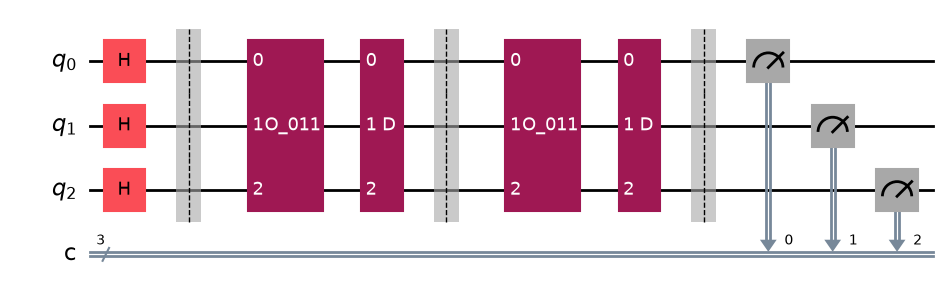
\includegraphics[width=0.8\textwidth]{imagenes/bloque4/e4_2_circuito_minimoK.png}
    \caption{Algoritmo de Grover para $N=8$ y $w=011$ con $k=2$ iteraciones. Cada iteración está formada por el oráculo $O$ y el operador de difusión $D$.}\label{fig:bloque4_e4_2_circuito}
\end{figure}

\textbf{Predicción.} Tras $k=2$ iteraciones, el estado marcado se mide con probabilidad $P_2=0{,}9453$ y cada uno de los otros siete estados con probabilidad $(1-P_2)/7=0{,}0078$. En 4096 disparos se esperan $3872$ conteos para $|011\rangle$ y $32$ para cada uno de los demás.
La comparación con la simulación se muestra en la Tabla~\ref{tab:bloque4_e4_2_hist} y en la Figura~\ref{fig:bloque4_e4_2_hist}.

\begin{table}[htbp]
    \centering
    \begin{tabular}{c|c|c|c|c}
    \hline
    Estado & $P$ teórica & $P$ simulada & Conteo teórico & Conteo simulado \\
    \hline
    \texttt{000} & 0,0078 & 0,0066 & 32 & 27 \\
    \texttt{001} & 0,0078 & 0,0081 & 32 & 33 \\
    \texttt{010} & 0,0078 & 0,0073 & 32 & 30 \\
    \texttt{011} & 0,9453 & 0,9475 & 3872 & 3881 \\
    \texttt{100} & 0,0078 & 0,0071 & 32 & 29 \\
    \texttt{101} & 0,0078 & 0,0100 & 32 & 41 \\
    \texttt{110} & 0,0078 & 0,0066 & 32 & 27 \\
    \texttt{111} & 0,0078 & 0,0068 & 32 & 28 \\
    \hline
    \end{tabular}
    \caption{Ejercicio 4.2: probabilidades y conteos teóricos y simulados con $k=2$ (4096 disparos).}\label{tab:bloque4_e4_2_hist}
\end{table}

\begin{figure}[h]
    \centering
    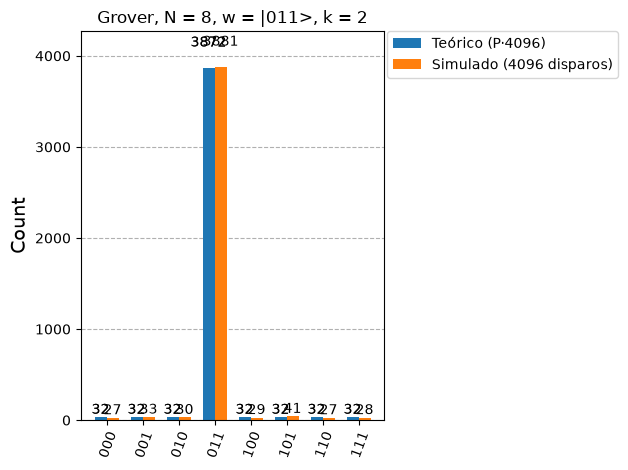
\includegraphics[width=0.5\textwidth]{imagenes/bloque4/e4_2_histograma_comparacion.png}
    \caption{Comparación del histograma simulado (4096 disparos) con la predicción teórica para $N=8$, $w=|011\rangle$ y $k=2$.}\label{fig:bloque4_e4_2_hist}
\end{figure}

\textbf{Resultado.} El histograma simulado reproduce la predicción: el estado marcado se mide con probabilidad 
$0{,}9475$ frente al valor teórico $0{,}9453$, y los siete restantes aparecen con frecuencias del orden de $0{,}7\%$.
El test $\chi^2$ de bondad de ajuste da un $p$-valor de $0{,}654$, compatible con la teoría al $5\%$.

%--------------------------------------------------------------------
\subsection{Ejercicio 4.3. Límite de probabilidad}
La probabilidad de éxito es $P_k(w)=\sin^2((2k+1)\theta)$, que solo vale 1 si $(2k+1)\theta=\pi/2+m\pi$ para algún entero $m$. Con $\theta=0{,}36137$ rad,
$$(2k+1)\theta=\frac{\pi}{2}\;\Longrightarrow\;k=\frac{1}{2}\Big(\frac{\pi}{2\theta}-1\Big)=1{,}673,$$
que no es un entero. Por tanto, en la \emph{primera} subida de $P_k$ no se alcanza el 1: el mejor entero es $k=2$, con $P_2=0{,}9453<0{,}99$. En esta primera subida \textbf{no es posible} llegar al $99\%$.

Sin embargo, $P_k$ es periódica en $k$ con periodo $\pi/(2\theta)=4{,}347$, que no es un entero, de modo que a medida que crece $k$ los valores $(2k+1)\theta$ recorren puntos distintos de cada ciclo y alguno puede caer muy cerca de $\pi/2+m\pi$.
Se tiene $P_k\ge0{,}99$ si y solo si $|(2k+1)\theta-(\pi/2+m\pi)|\le\arccos(\sqrt{0{,}99})=0{,}100$ rad. Para $k=2$ la diferencia es $0{,}236$ rad (no basta), pero para $\boldsymbol{k=6}$ se obtiene
$$13\,\theta=4{,}6978\ \text{rad}\ \text{frente a}\ \frac{3\pi}{2}=4{,}7124\ \text{rad},$$
es decir, una diferencia de solo $0{,}015$ rad y $P_6=0{,}99979$. La simulación lo confirma ($P_6=0{,}9993$). La Figura~\ref{fig:bloque4_e4_3} muestra $P_k$ frente a $k$ (teórica y simulada) y la Tabla~\ref{tab:bloque4_e4_3} recoge los valores.

\begin{figure}[h]
    \centering
    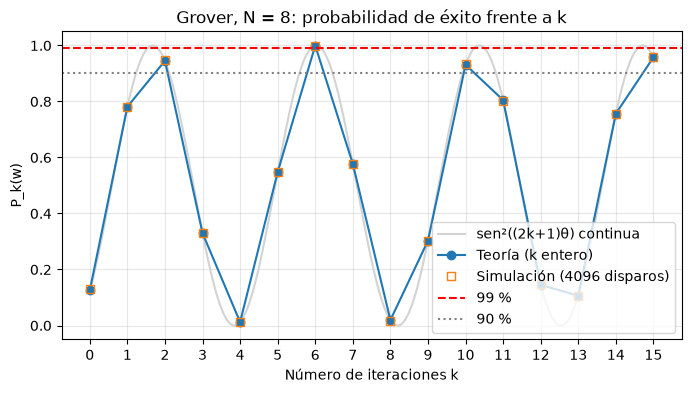
\includegraphics[width=0.8\textwidth]{imagenes/bloque4/e4_3_90percExito.png}
    \caption{Probabilidad de éxito $P_k(w)$ frente al número de iteraciones 
    $k$ para $N=8$: teoría (línea) y simulación con 4096 disparos (cuadrados). Se indican los umbrales del 
    $90\%$ y del $99\%$.}\label{fig:bloque4_e4_3}
\end{figure}

\begin{table}[htbp]
    \centering
    \begin{tabular}{c|c|c|c||c|c|c|c}
    \hline
    $k$ & $(2k+1)\theta$ & teórica & simulada & $k$ & $(2k+1)\theta$ & teórica & simulada \\
    \hline
    0 & 0,3614 & 0,1250 & 0,1313 & 8  & 6,1432  & 0,0195 & 0,0171 \\
    1 & 1,0841 & 0,7813 & 0,7795 & 9  & 6,8660  & 0,3029 & 0,3022 \\
    2 & 1,8068 & 0,9453 & 0,9475 & 10 & 7,5887  & 0,9313 & 0,9343 \\
    3 & 2,5296 & 0,3301 & 0,3318 & 11 & 8,3114  & 0,8049 & 0,8035 \\
    4 & 3,2523 & 0,0122 & 0,0115 & 12 & 9,0342  & 0,1450 & 0,1475 \\
    5 & 3,9750 & 0,5480 & 0,5483 & 13 & 9,7569  & 0,1063 & 0,1057 \\
    6 & 4,6978 & 0,9998 & 0,9993 & 14 & 10,4796 & 0,7566 & 0,7568 \\
    7 & 5,4205 & 0,5770 & 0,5784 & 15 & 11,2024 & 0,9578 & 0,9583 \\
    \hline
    \end{tabular}
    \caption{Ejercicio 4.3: probabilidad de éxito de Grover para $N=8$ y $k=0,\dots,15$.}\label{tab:bloque4_e4_3}
\end{table}

\textbf{Resultado.} Con $N=8$ el máximo de la primera subida es el $94{,}5\%$ ($k=2$), y ese es el límite si solo se consideran los primeros valores de $k$. Pero la probabilidad no está acotada por ese valor: como el periodo de $P_k$ no es entero,
sí es posible superar el $99\%$, y el primer $k$ que lo consigue es $k=6$ ($99{,}98\%$ teórico, $99{,}93\%$ simulado). En el rango estudiado ($k\le15$) es el único. Hay que tener en cuenta el coste: $k=6$ iteraciones implican 6 consultas al oráculo, más que las $\approx N/2=4$
consultas de media del algoritmo clásico, de modo que para un $N$ tan pequeño la ventaja cuadrática de Grover no se manifiesta; además, el resultado es muy sensible a $k$ ($P_5=0{,}548$ y $P_7=0{,}577$).
\section{Bloque 5}
\label{sec:bloque_5}


\setcounter{secnumdepth}{0}      % a partir de aquí, sin numerar
\section{Conclusiones}\label{sec:conclusiones}

En esta práctica se han implementado y simulado con Qiskit los elementos básicos de la algoritmia cuántica, desde los oráculos reversibles hasta la estimación cuántica de fase.
En todos los ejercicios la simulación ha coincidido, dentro de la fluctuación estadística de $4096$ disparos, con la predicción teórica calculada a mano o con \texttt{Statevector}.
Las conclusiones se organizan según los objetivos de la sección~\nameref{sec:objetivos}, seguidas de las ideas que atraviesan toda la memoria y de las limitaciones del trabajo.

%--------------------------------------------------------------------
\subsection{Conclusiones por objetivo}

\paragraph{Oráculos reversibles (Bloque 1 y ejercicio 2.5).} Una función booleana que no es reversible por sí sola (el AND, o una función $\{0,1\}^4\to\{0,1\}^4$ no inyectiva)
se implementa como la permutación $U_f|x\rangle|y\rangle=|x\rangle|y\oplus f(x)\rangle$, que es unitaria y cumple $U_f^2=I$. Con ella se construyeron el AND con una puerta Toffoli,
el XOR con dos CNOT, un oráculo de 3 bits con tres puertas multicontroladas y uno de 4 bits de entrada y 4 de salida con 32 puertas. En todas las entradas de cada oráculo
(4, 4, 8, 16 y 32 entradas en los ejercicios 1.1, 1.3, 1.4, 1.5 y 1.6) la salida coincide con la tabla de verdad con probabilidad 1 y la entrada se mide intacta.
La construcción importa para el coste: el oráculo lineal $f(x)=x_4\oplus x_3\oplus x_1$ necesita 3 CNOT, frente a las 16 puertas multicontroladas que requeriría la construcción por minitérminos.
Con la entrada en superposición, el paralelismo cuántico no equivale a leer toda la tabla: cada disparo devuelve una sola de las cuatro filas, que son equiprobables
(test $\chi^2$ con $p=0{,}979$ para el AND y $p=0{,}723$ para el XOR), y hacen falta en media $8{,}31$ disparos (simulado) frente a $25/3\approx8{,}33$ (teórico) para verlas todas.

\paragraph{Retroceso de fase (Bloque 2).} Si el objetivo de una puerta controlada está en un autovector, su autovalor aparece como \emph{fase relativa} en el control, y el objetivo no cambia.
Con $CP(\pi/4)$ el qubit de control gira $\pi/4$ alrededor del eje $z$ de la esfera de Bloch, mientras que la misma puerta $P(\pi/4)$ sin control es una fase global y no se observa.
Con el CNOT y el objetivo en $|{-}\rangle$ el control pasa de $|{+}\rangle$ a $|{-}\rangle$ y se mide $1$ con probabilidad 1, de modo que la medida \emph{revela} el autovalor de $X$;
con $X$ sin control se mide $0$ en ambos casos. En el barrido de $CP(\theta)$ se obtiene $P(q_0=1)=\sin^2(\theta/2)$ con una desviación máxima de $0{,}0047$ respecto a la simulación,
y se comprueba que $CP(\theta)^k=CP(k\theta)$, que es lo que permite implementar $U^{2^j}$ en QPE. En el ejercicio 2.5, con la ancilla en $|{-}\rangle$ el oráculo booleano se convierte
en un oráculo de fase, $U_f|x\rangle|{-}\rangle=(-1)^{f(x)}|x\rangle|{-}\rangle$, y el único autovalor $-1$ corresponde a $|1\rangle|{-}\rangle$.

\paragraph{Algoritmos de Deutsch, Deutsch-Jozsa y Bernstein-Vazirani (Bloque 3).} Con una sola consulta al oráculo, Deutsch separa las funciones constantes (se mide $0$) de las balanceadas (se mide $1$)
en los cuatro oráculos de una variable, frente a las 2 evaluaciones que necesita un algoritmo clásico. En Deutsch-Jozsa con $n=2$, la función constante da $|00\rangle$ y la función XOR
da $|11\rangle$ (balanceada), con 1 consulta frente a 3 en el peor caso clásico. La función AND no es ni constante ni balanceada: el resultado es una superposición que incluye $|00\rangle$ y otros estados, de modo que el algoritmo
no puede decidir. Esto ilustra que Deutsch-Jozsa depende de la promesa sobre $f$. Bernstein-Vazirani recupera las claves $a=1010$ y $a=1101$ con un único disparo y una sola consulta, frente a las 4 de un algoritmo clásico.
En el ejercicio E1 la medida $01$ indica que la función es balanceada, y la tabla de verdad obtenida ($f=\overline{x_1}$) es coherente con el análisis como función afín, con $s=(0,1)$ y $b=1$.

\paragraph{Algoritmo de Grover (Bloque 4).} Para $N=8$ y $w=011$, una iteración lleva la amplitud del estado marcado de $-0{,}354$ a $5/(2\sqrt8)\approx0{,}884$ y su probabilidad de $0{,}125$ a $0{,}781$, tal como se calculó a mano.
El mínimo $k$ con al menos un $90\%$ de éxito es $k=2$: $P_2=0{,}9453$ teórica y $0{,}9475$ simulada, con $3872$ y $3881$ conteos para $|011\rangle$ ($\chi^2$ con $p=0{,}654$). Iterar más no mejora el resultado:
$P_3=0{,}330$, porque cada iteración gira el estado un ángulo $2\theta$ y con $k=3$ se sobrepasa el estado marcado. Alcanzar el $99\%$ no es posible en la primera subida ($k=1{,}673$ no es entero),
pero sí con $k=6$, que da $P_6=0{,}9998$ teórica y $0{,}9993$ simulada. El resultado es muy sensible a $k$ ($P_5=0{,}548$ y $P_7=0{,}577$). Con $k=2$ bastan 2 consultas al oráculo frente a las $\approx N/2=4$ de media clásicas,
pero con $k=6$ ya se necesitan más que las clásicas, de modo que para un $N$ tan pequeño solo hay ahorro de consultas en el primer caso.

\paragraph{Estimación cuántica de fase (Bloque 5).} Cuando la fase es diádica la estimación es exacta y determinista: la puerta $S$ con $t=2$ da $m=1$ ($\tilde\varphi=1/4$), y $\theta=3/32$ con $t=5$ da $m=3$ con error nulo.
Cuando no lo es, el error queda acotado por $2^{-(t+1)}$: para $\theta=1/3$ y $t=3$ se obtiene $m=3$, $\tilde\varphi=0{,}375$ y un error de $0{,}042<0{,}0625$, con $P(3)=0{,}6878$ teórica y $2826/4096\approx0{,}690$ medida.
Al aumentar $t$ el error de $\theta=1/3$ se reduce a la mitad por cada qubit ($0{,}02083$, $0{,}01042$ y $0{,}00521$ para $t=4,5,6$), y $t=6$ es el menor valor que garantiza un error inferior a $0{,}01$.
Para $\theta=2/5$ pasar de $t=2$ a $t=5$ reduce el error de $0{,}1$ a $0{,}00625$ (un factor $16$). En cambio, la probabilidad del pico \emph{no} tiende a 1 sino a $27/(4\pi^2)\approx0{,}684$, porque
$1/3$ queda siempre a $1/3$ de marca de la rejilla $m/2^t$: más qubits mejoran la estimación, pero no la probabilidad de obtener un único valor de $m$. Con el operador diagonal de dos fases ($t=6$)
el autovector $|1\rangle$ da $m=24$ sin error y $|0\rangle$ da $m=18$ con error $0{,}00625$, porque $\varphi_0=0{,}275$ no es diádica. Con una superposición $c_0|0\rangle+c_1|1\rangle$ aparecen los dos picos, $m=18$ y $m=24$,
con un peso proporcional a $|c_a|^2$ ($0{,}461$ observado frente a $0{,}458$ previsto para $m=18$ y $0{,}206$ frente a $0{,}202$ para $m=24$ con $|c_0|^2=0{,}8$), y medir el registro de conteo equivale a medir $U$:
el estado $|\psi\rangle$ colapsa sobre uno de sus autovectores.

%--------------------------------------------------------------------
\subsection{Ideas transversales}

\paragraph{El retroceso de fase como hilo conductor.} El mismo mecanismo aparece en los Bloques 3, 4 y 5: la ancilla en $|{-}\rangle$ convierte el oráculo booleano en un oráculo de fase $(-1)^{f(x)}$ en Deutsch, Deutsch-Jozsa y Bernstein-Vazirani,
el oráculo de Grover marca el estado con un signo $-1$ y QPE lee en el registro de conteo la fase del autovalor de $U$. Los ejercicios del Bloque 2, con un solo control y un solo autovector, son la versión mínima de todos ellos.

\paragraph{Concordancia entre teoría y simulación.} La Tabla~\ref{tab:conclusiones_resumen} reúne las comprobaciones cuantitativas principales. Todos los tests $\chi^2$ dan $p>0{,}05$ y las desviaciones
observadas son del orden del ruido estadístico típico $1/\sqrt{4096}\approx0{,}016$ o menores. Se ha usado \texttt{Statevector} cuando se necesitaban amplitudes y fases exactas, y \texttt{AerSimulator} cuando el resultado pedido era una medida.

\begin{table}[htbp]
    \centering
    {\small\setlength{\tabcolsep}{4pt}
    \begin{tabular}{c|p{0.40\textwidth}|c|c}
    \hline
    Bloque & Magnitud & Teórico & Simulado \\
    \hline
    1 & Disparos medios para ver las 4 filas (ej.~1.2) & $8{,}33$ & $8{,}31$ \\
    2 & $P(q_0=1)$ para $\theta=\pi/4$ (ej.~2.4) & $0{,}1464$ & $0{,}1511$ \\
    4 & $P_2$ de Grover, $N=8$ & $0{,}9453$ & $0{,}9475$ \\
    4 & $P_6$ de Grover, $N=8$ & $0{,}9998$ & $0{,}9993$ \\
    5 & $P(m=3)$ en QPE con $t=3$, $\theta=1/3$ & $0{,}6878$ & $0{,}690$ \\
    5 & Pico de QPE para $\theta=1/3$, $t=4,5,6$ & $0{,}685;\ 0{,}684;\ 0{,}684$ & $0{,}683;\ 0{,}686;\ 0{,}682$ \\
    5 & $P(m=18)$ y $P(m=24)$ con $|c_0|^2=0{,}8$ & $0{,}458;\ 0{,}202$ & $0{,}461;\ 0{,}206$ \\
    \hline
    \end{tabular}}
    \caption{Resumen de las comprobaciones teoría--simulación más relevantes.}\label{tab:conclusiones_resumen}
\end{table}

\paragraph{Ventaja cuántica y sus límites.} Los algoritmos de los Bloques 3 y 4 resuelven el problema con menos consultas que el caso clásico (1 frente a 2, 3 y 4 en Deutsch, Deutsch-Jozsa y Bernstein-Vazirani con $n=1,2,4$),
pero la ventaja depende de las hipótesis del problema (la promesa de Deutsch-Jozsa, la forma lineal de Bernstein-Vazirani) y del tamaño: en Grover con $N=8$ se pierde cuando se exige el $99\%$ de éxito.

\paragraph{Convenios de bits y reproducibilidad.} Los resultados se leen correctamente solo si se conoce el convenio de orden de los bits. Se ha seguido el convenio \textit{little-endian} de Qiskit en todos los bloques, salvo en el ejercicio 3.3 y en el E1,
donde se invierte la asignación de bits clásicos y está indicado en cada caso (sección~\nameref{sec:entorno_convenciones}). Con la semilla del simulador fijada, el cuaderno reproduce las figuras y las tablas de la memoria.

%--------------------------------------------------------------------
\subsection{Limitaciones y trabajo futuro}

Todas las simulaciones son ideales y sin ruido, por lo que resultados como la probabilidad exacta 1 de los oráculos o los picos limpios de QPE no son extrapolables a un dispositivo real.
Además, los tamaños son pequeños ($n\le4$ en los oráculos, $N=8$ en Grover, $t\le6$ en la mayor parte de QPE), y la comparación de consultas entre algoritmos cuánticos y clásicos es teórica, no una medida de tiempo.
Como continuación natural se proponen:
\begin{itemize}
    \item introducir un modelo de ruido en \texttt{AerSimulator} o ejecutar en hardware real, y medir cómo afectan la profundidad del circuito y el número de puertas multicontroladas a Grover y a QPE;
    \item extender Grover a varios estados marcados y a un número de soluciones desconocido, y ver cómo cambia el número óptimo de iteraciones;
    \item reducir el coste de QPE con variantes que usan menos qubits de conteo, como la estimación iterativa de fase, y relacionarla con aplicaciones como la factorización de Shor.
\end{itemize}

\section{Apéndice}\label{sec:apendice}

Este apéndice recoge las partes significativas del código del cuaderno, ordenadas por bloque: las funciones auxiliares, la construcción de los oráculos y de los circuitos de cada algoritmo,
y las comprobaciones que contrastan la simulación con la teoría. Para no repetir código se muestra un caso representativo cuando varios ejercicios usan el mismo patrón
(por ejemplo, solo la clave $a=1010$ de Bernstein-Vazirani), y se han omitido las instrucciones de dibujo y de impresión por pantalla (\texttt{display}, \texttt{draw}, \texttt{plot\_histogram}, \texttt{print} de tablas).
El cuaderno completo reproduce todas las figuras y tablas de la memoria; los listados siguen la convención \textit{little-endian} de Qiskit, salvo donde se indica lo contrario en cada bloque.

\lstset{
    language=Python,
    basicstyle=\ttfamily\footnotesize,
    keywordstyle=\bfseries,
    commentstyle=\itshape,
    numbers=left,
    numberstyle=\tiny,
    numbersep=6pt,
    xleftmargin=1.6em,
    frame=single,
    framesep=3pt,
    breaklines=true,
    breakindent=1.5em,
    postbreak=\mbox{$\hookrightarrow$\space},
    showstringspaces=false,
    tabsize=4,
    captionpos=b,
    aboveskip=1.2ex,
    belowskip=1.2ex,
    literate=
        {á}{{\'a}}1 {é}{{\'e}}1 {í}{{\'i}}1 {ó}{{\'o}}1 {ú}{{\'u}}1 {ñ}{{\~n}}1
        {Á}{{\'A}}1 {É}{{\'E}}1 {Í}{{\'I}}1 {Ó}{{\'O}}1 {Ú}{{\'U}}1 {Ñ}{{\~N}}1
        {¿}{{?`}}1 {¡}{{!`}}1 {·}{{$\cdot$}}1 {θ}{{$\theta$}}1 {π}{{$\pi$}}1,
}
\renewcommand{\lstlistingname}{Código}

\subsection{Configuración común}

Parámetros globales y función de simulación usados en todos los bloques. La semilla se fija en el simulador (\texttt{seed\_simulator}), tanto en el constructor como en cada ejecución, porque es la única que controla el muestreo de Aer.

\begin{lstlisting}[caption={Importaciones principales, semilla, número de disparos, simulador y función de simulación (todos los bloques).},label={lst:config}]
from qiskit import QuantumRegister, QuantumCircuit, generate_preset_pass_manager
from qiskit import transpile
from qiskit_aer import AerSimulator
from qiskit.circuit.library import *
from qiskit.circuit import Gate
import numpy as np
from qiskit.quantum_info import Statevector, Pauli, Operator
from tabulate import tabulate
import matplotlib.pyplot as plt
from scipy.stats import chisquare, chi2

seed = 98
shots = 4096
np.random.seed(seed)
random.seed(seed)
sim = AerSimulator(seed_simulator=seed)  
RESULTS = {'tables': {}, 'figures': {}, 'metrics': {}}

def simular(qc, n_shots=shots, memory=False):
    """Ejecuta qc en AerSimulator (semilla fija). Devuelve los counts y, si memory=True,
    también la lista de resultados disparo a disparo."""
    res = sim.run(transpile(qc, sim), shots=n_shots, memory=memory, seed_simulator=seed).result()
    if memory:
        return res.get_counts(), res.get_memory()
    return res.get_counts()
\end{lstlisting}

\subsection{Bloque 1: oráculos booleanos reversibles}

El oráculo $U_f|x\rangle|y\rangle=|x\rangle|y\oplus f(x)\rangle$ se construye a partir de la tabla de verdad con una \texttt{MCXGate} por cada fila con salida $1$; las funciones AND, XOR y lineal se implementan directamente con Toffoli y CNOT.

\begin{lstlisting}[caption={Construcción de oráculos por minitérminos y casos particulares (ejercicios 1.1, 1.3, 1.4 y 1.6).},label={lst:b1_oraculos}]
def oraculo_booleano(tabla, nombre_in='x', nombre_out='y'):
    """Oráculo U_f|x>|y> = |x>|y XOR f(x)> para una tabla {'x_{n-1}..x_0': 'f_{m-1}..f_0'}.
    Entrada x_j en el qubit j; el bit f_j se suma al qubit n+j.
    Se añade una MCXGate por cada entrada x y por cada bit de salida f_j = 1; los controles
    actúan sobre |1> o sobre |0> según los bits de x (ctrl_state = x)."""
    n_in = len(next(iter(tabla)))
    n_out = len(next(iter(tabla.values())))
    entrada = QuantumRegister(n_in, nombre_in)
    salida = QuantumRegister(n_out, nombre_out)
    qc = QuantumCircuit(entrada, salida, name='U_f')
    for x, fx in tabla.items():
        for j, bit in enumerate(fx[::-1]):            # bit f_j de la salida
            if bit == '1':
                qc.append(MCXGate(n_in, ctrl_state=x), list(entrada) + [salida[j]])
    return qc

# Oráculo: Toffoli con controles q0 (a0), q1 (a1) y objetivo q2 (ancilla y)
tabla_and = {'00': '0', '01': '0', '10': '0', '11': '1'}     # a1a0 -> a1 AND a0

oraculo_and = QuantumCircuit(3, name='U_AND')
oraculo_and.ccx(0, 1, 2)

tabla_xor = {'00': '0', '01': '1', '10': '1', '11': '0'}     # a1a0 -> a1 XOR a0

oraculo_xor = QuantumCircuit(3, name='U_XOR')
oraculo_xor.cx(0, 2)
oraculo_xor.cx(1, 2)

def oraculo_con_X(tabla):
    n_in = len(next(iter(tabla)))
    qc = QuantumCircuit(n_in + 1, name='U_f (con X)')
    for x, fx in tabla.items():
        if fx == '1':
            ceros = [j for j, b in enumerate(x[::-1]) if b == '0']
            if ceros:
                qc.x(ceros)
            qc.mcx(list(range(n_in)), n_in)
            if ceros:
                qc.x(ceros)
            qc.barrier()
    return qc

def oraculo_lineal(a, nombre_in='x', nombre_out='y'):
    """Oráculo de f(x) = a·x (mod 2). a = 'a_{n-1}...a_0'; el bit a_i controla un CNOT desde q_i a la ancilla."""
    n = len(a)
    entrada = QuantumRegister(n, nombre_in)
    salida = QuantumRegister(1, nombre_out)
    qc = QuantumCircuit(entrada, salida, name=f'U_f (a={a})')
    for i, bit in enumerate(a[::-1]):
        if bit == '1':
            qc.cx(entrada[i], salida[0])
    return qc

def tabla_lineal(a):
    """Tabla de verdad teórica de f(x) = a·x (mod 2): paridad de los bits de a AND x."""
    n = len(a)
    return {format(x, f'0{n}b'): str(bin(x & int(a, 2)).count('1') % 2) for x in range(2 ** n)}
\end{lstlisting}

La verificación prepara cada entrada con puertas $X$, aplica el oráculo, mide todos los qubits y compara con la tabla teórica; además se comprueba que la matriz del circuito es la permutación teórica y que $U_f^2=I$.

\begin{lstlisting}[caption={Verificación del oráculo con entradas clásicas y comprobación matricial.},label={lst:b1_verificacion}]
def circuito_entrada_clasica(oraculo, x):
    """Prepara |x> con puertas X, aplica el oráculo y mide todos los qubits."""
    n = oraculo.num_qubits
    qc = QuantumCircuit(n, n)
    for j, bit in enumerate(x[::-1]):                 # x_j en el qubit j
        if bit == '1':
            qc.x(j)
    qc.barrier()
    qc.compose(oraculo, range(n), inplace=True)
    qc.barrier()
    qc.measure(range(n), range(n))
    return qc

def verificar_oraculo(oraculo, tabla, etiqueta='x'):
    """Simula el oráculo para cada entrada clásica y compara con la tabla teórica.
    La cadena medida es 'f_{m-1}..f_0 x_{n-1}..x_0'."""
    n_out = len(next(iter(tabla.values())))
    filas, todo_ok = [], True
    for x, fx in tabla.items():
        counts = simular(circuito_entrada_clasica(oraculo, x))
        medido = max(counts, key=counts.get)
        salida, entrada = medido[:n_out], medido[n_out:]
        ok = (salida == fx) and (entrada == x) and (len(counts) == 1)
        todo_ok &= ok
        filas.append([x, fx, salida, entrada, counts[medido] / shots, 'OK' if ok else 'ERROR'])
    cabecera = [etiqueta, 'f(x) teórica', 'f(x) simulada', 'x tras U_f', 'Probabilidad', 'Estado']
    print(tabulate(filas, headers=cabecera, tablefmt='github'))
    print(f'\n{sum(f[-1] == "OK" for f in filas)}/{len(filas)} entradas correctas'
          f' -> {"el oráculo es correcto" if todo_ok else "HAY ERRORES"}')
    return filas

def matriz_oraculo_teorica(tabla):
    """Matriz (permutación) de |x>|y> -> |x>|y XOR f(x)> con el orden de bits de Qiskit."""
    n_in = len(next(iter(tabla)))
    n_out = len(next(iter(tabla.values())))
    dim = 2 ** (n_in + n_out)
    U = np.zeros((dim, dim))
    for x, fx in tabla.items():
        for y in range(2 ** n_out):
            columna = (y << n_in) | int(x, 2)
            fila = ((y ^ int(fx, 2)) << n_in) | int(x, 2)
            U[fila, columna] = 1
    return U

def comprobar_matriz(oraculo, tabla):
    """Comprueba que la matriz del circuito es la de U_f y que U_f^2 = I."""
    U = Operator(oraculo).data
    print('Matriz del circuito = matriz teórica de U_f :', np.allclose(U, matriz_oraculo_teorica(tabla)))
    print('U_f es su propio inverso (U_f^2 = I)         :', np.allclose(U @ U, np.eye(U.shape[0])))
\end{lstlisting}

Para el paralelismo cuántico (ejercicios 1.2 y 1.3) se aplican $H$ a las entradas antes del oráculo. El experimento de un solo disparo usa una semilla distinta en cada ejecución y cuenta los disparos necesarios para ver las cuatro filas.

\begin{lstlisting}[caption={Entrada en superposición y experimento de disparos (ejercicios 1.2 y 1.3).},label={lst:b1_superposicion}]
def circuito_superposicion(oraculo, n_in, medir=True):
    """H en los n_in qubits de entrada, oráculo y (opcionalmente) medida de todos los qubits."""
    n = oraculo.num_qubits
    qc = QuantumCircuit(n, n) if medir else QuantumCircuit(n)
    qc.h(range(n_in))
    qc.barrier()
    qc.compose(oraculo, range(n), inplace=True)
    if medir:
        qc.barrier()
        qc.measure(range(n), range(n))
    return qc

def probs_teoricas(tabla):
    """Predicción analítica: todas las filas (f(x), x) equiprobables. Clave = 'f x'."""
    return {fx + x: 1 / len(tabla) for x, fx in tabla.items()}

def disparos_hasta_tabla_completa(memoria, n_filas):
    """Con la memoria disparo a disparo, cuenta cuántos disparos consecutivos hacen falta
    para haber visto las n_filas salidas distintas (se reinicia al completarlas)."""
    longitudes, vistos, n = [], set(), 0
    for m in memoria:
        n += 1
        vistos.add(m)
        if len(vistos) == n_filas:
            longitudes.append(n)
            vistos, n = set(), 0
    return longitudes

qc_t = transpile(qc_sup_and, sim)
unico = [next(iter(sim.run(qc_t, shots=1, seed_simulator=1000 + s).result().get_counts())) for s in range(10)]
_, mem = simular(qc_sup_and, n_shots=40, memory=True)
_, mem_largo = simular(qc_sup_and, n_shots=50000, memory=True)
longitudes = disparos_hasta_tabla_completa(mem_largo, len(tabla_and))

_, memoria = simular(qc_sup_and, n_shots=shots, memory=True)
longitudes = disparos_hasta_tabla_completa(memoria, n_filas)
teoria = n_filas * sum(1 / k for k in range(1, n_filas + 1))
\end{lstlisting}

\subsection{Bloque 2: retroceso de fase}

Todos los ejercicios de este bloque aplican las puertas una a una y guardan el \texttt{Statevector} tras cada paso. El vector de Bloch de un qubit se calcula con los valores esperados de $X$, $Y$ y $Z$, lo que vale también para qubits entrelazados.

\begin{lstlisting}[caption={Evolución paso a paso, vector de Bloch y probabilidad de medir $q_0=1$.},label={lst:b2_utilidades}]
def evolucion(n, pasos):
    """Aplica uno a uno los pasos (etiqueta, funcion(qc)) a un circuito de n qubits sin medidas
    y guarda el Statevector tras cada uno. Devuelve (circuito, [(etiqueta, Statevector)])."""
    qc = QuantumCircuit(n)
    salida = [('Estado inicial', Statevector(qc))]
    for etiqueta, fn in pasos:
        fn(qc)
        salida.append((etiqueta, Statevector(qc)))
    return qc, salida

def vector_bloch(psi, qubit):
    """(<X>, <Y>, <Z>) del qubit indicado (vale también para qubits entrelazados)."""
    return tuple(float(np.real(psi.expectation_value(Pauli(p), [qubit]))) for p in 'XYZ')

def prob_q0_uno(counts):
    """P(q0 = 1) a partir de counts con cadena 'c1c0' (el bit de la derecha es q0)."""
    return sum(v for k, v in counts.items() if k[-1] == '1') / sum(counts.values())
\end{lstlisting}

\begin{lstlisting}[caption={Ejercicio 2.1: $CP(\pi/4)$ con comprobación del cálculo a mano y caso sin control.},label={lst:b2_cp}]
s = 1 / np.sqrt(2)
pasos_21 = [('Tras H(q0)', lambda qc: qc.h(0)),
            ('Tras X(q1)', lambda qc: qc.x(1)),
            ('Tras CP(pi/4), control q0 y objetivo q1', lambda qc: qc.cp(np.pi / 4, 0, 1))]
qc_21, est_21 = evolucion(2, pasos_21)
# Estados calculados a mano, en el orden [|00>, |01>, |10>, |11>] = |q1 q0>
a_mano_21 = [np.array([1, 0, 0, 0]),
             np.array([s, s, 0, 0]),
             np.array([0, 0, s, s]),
             np.array([0, 0, s, s * np.exp(1j * np.pi / 4)])]
for (etiqueta, psi), v in zip(est_21, a_mano_21):
    print(f'{etiqueta:42s} coincide con el cálculo a mano: {np.allclose(psi.data, v)}')

pasos_21c = [('Tras H(q0)', lambda qc: qc.h(0)),
             ('Tras X(q1)', lambda qc: qc.x(1)),
             ('Tras P(pi/4) sobre q1 (sin control)', lambda qc: qc.p(np.pi / 4, 1))]
qc_21c, est_21c = evolucion(2, pasos_21c)
antes, despues = est_21c[2][1], est_21c[3][1]
i = np.argmax(np.abs(antes.data))
print('Factor entre el estado de después y el de antes de P(π/4):', np.round(despues.data[i] / antes.data[i], 4),
      f'  (= e^(iπ/4) = {np.round(np.exp(1j*np.pi/4), 4)})')
print('¿Mismo estado salvo fase global (Statevector.equiv)?      :', despues.equiv(antes))
\end{lstlisting}

\begin{lstlisting}[caption={Ejercicio 2.2: pasos del circuito con CNOT o con $X$ sobre $q_1$.},label={lst:b2_cnot}]
def pasos_22(q1_menos, puerta):
    def preparar(qc):
        qc.h(0)
        if q1_menos:
            qc.x(1)
        qc.h(1)
    def compuerta(qc):
        if puerta == 'cx':
            qc.cx(0, 1)
        else:
            qc.x(1)
    def volver(qc):
        qc.h([0, 1])
    nombre_q1 = '|->' if q1_menos else '|+>'
    nombre_p = 'CNOT(q0->q1)' if puerta == 'cx' else 'X(q1)'
    return [(f'Tras preparar q0=|+>, q1={nombre_q1}', preparar),
            (f'Tras {nombre_p}', compuerta),
            ('Tras H en q0 y q1', volver)]

final_mano_22 = {('cx', False): [1, 0, 0, 0],      # |00>
                 ('cx', True):  [0, 0, 0, 1],      # |11>
                 ('x',  False): [1, 0, 0, 0],      # |00>
                 ('x',  True):  [0, 0, -1, 0]}     # -|10>  (q1=1, q0=0, signo global)
\end{lstlisting}

\begin{lstlisting}[caption={Ejercicios 2.3 y 2.4: pasos con $CP(\theta)$, barrido de $\theta$ y comprobación de $CP(\theta)^k=CP(k\theta)$.},label={lst:b2_barrido}]
def pasos_cp(theta):
    return [('(1) Tras X(q1): psi', lambda qc: qc.x(1)),
            ("(2) Tras H(q0): psi'", lambda qc: qc.h(0)),
            ("(3) Tras CP(θ): psi''", lambda qc: qc.cp(theta, 0, 1)),
            ("(4) Tras H(q0): psi'''", lambda qc: qc.h(0))]

def circuito_cp_medido(qc_sin_medidas):
    qc = QuantumCircuit(2, 2)
    qc.compose(qc_sin_medidas, inplace=True)
    qc.measure([0, 1], [0, 1])
    return qc

ks = np.arange(1, 8)
filas_24, bloch3, bloch4, p1_sim_24 = [], [], [], []
for k in ks:
    theta = k * np.pi / 4
    qc_, est_ = evolucion(2, pasos_cp(theta))
    v3, v4 = vector_bloch(est_[3][1], 0), vector_bloch(est_[4][1], 0)
    bloch3.append(v3); bloch4.append(v4)
    p1 = prob_q0_uno(simular(circuito_cp_medido(qc_)))
    p1_sim_24.append(p1)
    ok3 = np.allclose(v3, (np.cos(theta), np.sin(theta), 0))
    ok4 = np.allclose(v4, (0, -np.sin(theta), np.cos(theta)))

# Dos CP(pi/2) encadenadas frente a una CP(pi)
doble = QuantumCircuit(2); doble.cp(np.pi / 2, 0, 1); doble.cp(np.pi / 2, 0, 1)
unica = QuantumCircuit(2); unica.cp(np.pi, 0, 1)
print('Operator(CP(π/2) · CP(π/2)) == Operator(CP(π)):', Operator(doble).equiv(Operator(unica)))
ok = all(np.allclose(np.linalg.matrix_power(Operator(CPhaseGate(th)).data, kk), Operator(CPhaseGate(kk * th)).data)
         for th in np.linspace(0.1, 3, 8) for kk in range(1, 9))
print('CP(θ)^k = CP(kθ) para 8 valores de θ y k = 1..8:', ok)

qc_c = QuantumCircuit(2, 2); qc_c.x(1); qc_c.h(0)
qc_c.cp(np.pi / 2, 0, 1); qc_c.cp(np.pi / 2, 0, 1)
qc_c.h(0); qc_c.measure([0, 1], [0, 1])
print('P(q0=1) con dos CP(π/2):', prob_q0_uno(simular(qc_c)), '(teoría sin^2(π/2) = 1)')
\end{lstlisting}

\begin{lstlisting}[caption={Ejercicio 2.5: oráculo $f(x)=x$ y cálculo de los autovalores $\lambda=\langle\psi_{in}|\psi_{out}\rangle$.},label={lst:b2_oraculo}]
uf_25 = QuantumCircuit(2, name='U_f')      # q0 = x (dato), q1 = y (ancilla)
uf_25.cx(0, 1)

filas_25b = []
for x in (0, 1):
    for a in ('+', '-'):
        psi_in = Statevector.from_label(a + str(x))          # etiqueta = 'q1 q0' = 'ancilla dato'
        psi_out = psi_in.evolve(uf_25)
        lam = psi_in.inner(psi_out)                          # <psi_in|psi_out>
        es_autovector = np.allclose(psi_out.data, lam * psi_in.data)
        lam_teo = 1 if a == '+' else (-1) ** x
        filas_25b.append([f'|{x}>|{a}>', f'{lam.real:+.3f}{lam.imag:+.3f}j', lam_teo, es_autovector,
                          'OK' if (es_autovector and np.isclose(lam, lam_teo)) else 'ERROR'])

# Retroceso de fase: con el dato en |+> y la ancilla en |->, U_f lleva el dato a |->
psi_in = Statevector.from_label('-+')
psi_out = psi_in.evolve(uf_25)
print('\nU_f |+>|->  ==  |->|->  :', psi_out.equiv(Statevector.from_label('--')))
\end{lstlisting}

\subsection{Bloque 3: Deutsch, Deutsch-Jozsa y Bernstein-Vazirani}

En los tres algoritmos la ancilla se prepara en $|1\rangle$ y se aplican $H$ a todos los qubits antes y después del oráculo. En el ejercicio 3.3 y en el ejercicio E1 se invierte la asignación de bits clásicos en la medida (véase la sección «\nameref{sec:entorno_convenciones}»).

\begin{lstlisting}[caption={Ejercicio 3.1: oráculos de una variable y circuito de Deutsch.},label={lst:b3_deutsch}]
def oraculo(qc, tipo):
    if tipo == "a":          # f(x) = 0 -> identidad
        pass
    elif tipo == "b":        # f(x) = 1 -> X sobre la ancilla
        qc.x(1)
    elif tipo == "c":        # f(x) = x -> CNOT
        qc.cx(0, 1)
    elif tipo == "d":        # f(x) = NOT x -> CNOT + X
        qc.cx(0, 1)
        qc.x(1)

def deutsch(tipo):
    qc = QuantumCircuit(2, 1)
    qc.x(1)                  # ancilla en |1>
    qc.h([0, 1])
    qc.barrier()
    oraculo(qc, tipo)
    qc.barrier()
    qc.h(0)
    qc.measure(0, 0)
    return qc

deutsch_qcs = {}
for t in "abcd":
    qc = deutsch(t)
    deutsch_qcs[t] = qc
\end{lstlisting}

\begin{lstlisting}[caption={Ejercicio 3.2: oráculos de dos variables y circuito de Deutsch-Jozsa.},label={lst:b3_dj}]
def oraculos3_2(tipo):
    qc = QuantumCircuit(3, name = f'oraculo {tipo}')
    if tipo == "a":
        pass
    elif tipo == "b":
        qc.cx(0, 2)
        qc.cx(1, 2)
    else: #apartado c)
        qc.ccx(0, 1, 2)
    return qc.to_gate()

def deutsch_jozsa(oraculo, n = 2):
    qc = QuantumCircuit(n + 1, n)
    qc.x(n)
    qc.h(range(n + 1))
    
    qc.append(oraculo, range(n + 1))
    qc.h(range(n + 1))
    qc.measure(range(n), range(n))
    return qc
\end{lstlisting}

\begin{lstlisting}[caption={Ejercicio 3.3: Bernstein-Vazirani con clave $a=1010$ y medida con el orden de bits invertido.},label={lst:b3_bv}]
#Construyo oraculo para clave oculta a = 1010
oraculo_a1 = QuantumCircuit(5, name = "oraculo_a1")
oraculo_a1.cx(0, 4)
oraculo_a1.cx(2, 4)
oraculoa1_gate = oraculo_a1.to_gate()

bvazirani_a1 = QuantumCircuit(5, 4, name = "circuito_bernstein_vazirani")
bvazirani_a1.x(4)
bvazirani_a1.h(range(5))
bvazirani_a1.barrier()
bvazirani_a1.append(oraculoa1_gate, range(5))
bvazirani_a1.barrier()
bvazirani_a1.h(range(5))
bvazirani_a1.measure(range(4), range(3, -1, -1)) #Invierto los bits de medida
bvazirani_a1.measure(range(4), range(3, -1, -1)) #Invierto los bits de medida
counts = sim.run(transpile(bvazirani_a1, sim), shots=1).result().get_counts()
\end{lstlisting}

\begin{lstlisting}[caption={Ejercicio E1: oráculo dado, circuito de Deutsch-Jozsa y tabla de verdad de $f$.},label={lst:b3_e1}]
# Construyo el oraculo
dj_f = QuantumCircuit(3, name = "DJ_F")
dj_f.x([0, 1])
dj_f.ccx(0, 1, 2)
dj_f.x([0, 1])

dj_f.x(1)
dj_f.ccx(0, 1, 2)
dj_f.x(1)

# Implemento el circuito
e1dj = QuantumCircuit(3, 2)
e1dj.x(2)
e1dj.h([0, 1, 2])
e1dj.append(oraculo_djf, [0, 1, 2])
e1dj.h([0, 1])

e1dj.measure([0, 1], [1, 0])

counts = sim.run(transpile(e1dj, sim), shots = shots).result().get_counts()

def init_circuit (qc, valor):
    if valor == 0:
        pass
    elif valor == 1:
        qc.x(1)
    elif valor == 2:
        qc.x(0)
    else:
        qc.x([0, 1])

for i in range(4):
    qc = QuantumCircuit(3, 1)
    init_circuit(qc, i)
    qc.append(oraculo_djf, [0, 1, 2])
    qc.measure(2, 0)

    counts = sim.run(transpile(qc, sim), shots = shots).result().get_counts()
\end{lstlisting}

\subsection{Bloque 4: algoritmo de Grover}

El oráculo de fase se construye con una $Z$ multicontrolada ($H\cdot\mathrm{MCX}\cdot H$) rodeada de puertas $X$ en los qubits donde $w$ tiene un $0$. El circuito de difusión produce $-D$, por lo que se le añade una fase global $\pi$.

\begin{lstlisting}[caption={Oráculo de fase, operador de difusión, circuito de Grover y probabilidad teórica $P_k$.},label={lst:b4_grover}]
# Convenio: w = 'x_{n-1}...x_0' con x_j en el qubit q_j (Qiskit, little-endian).
# El estado |w> es el índice int(w, 2) del vector de estado.
def z_multicontrolada(qc, n):
    """Z con n-1 controles sobre q_{n-1}: H · MCX · H. Cambia el signo solo de |1...1>."""
    if n == 1:
        qc.z(0)
    else:
        qc.h(n - 1)
        qc.mcx(list(range(n - 1)), n - 1)
        qc.h(n - 1)

def oraculo_fase(w):
    """O|x> = -|x> si x = w, |x> en otro caso. Se rodean con X los qubits en los que w tiene un 0."""
    n = len(w)
    qc = QuantumCircuit(n, name=f'O_{w}')
    ceros = [j for j, b in enumerate(w[::-1]) if b == '0']
    if ceros: qc.x(ceros)
    z_multicontrolada(qc, n)
    if ceros: qc.x(ceros)
    return qc

def difusion(n):
    """D = 2|s><s| - I = H^n (2|0><0| - I) H^n.
    X^n · MCZ · X^n = I - 2|0><0|, así que H^n X^n MCZ X^n H^n = -D; la fase global pi lo convierte exactamente en D."""
    qc = QuantumCircuit(n, name='D')
    qc.h(range(n)); qc.x(range(n))
    z_multicontrolada(qc, n)
    qc.x(range(n)); qc.h(range(n))
    qc.global_phase = np.pi
    return qc

def grover(w, k, medir=True):
    """H^n, k iteraciones G = D·O y (opcional) medida de los n qubits."""
    n = len(w)
    qc = QuantumCircuit(n, n) if medir else QuantumCircuit(n)
    qc.h(range(n))
    O, D = oraculo_fase(w).to_gate(), difusion(n).to_gate()
    for _ in range(k):
        qc.barrier()
        qc.append(O, range(n))
        qc.append(D, range(n))
    if medir:
        qc.barrier()
        qc.measure(range(n), range(n))
    return qc

def p_teorica(k, N, M=1):
    """P_k(w) = sen^2((2k+1) theta), sen theta = sqrt(M/N)."""
    theta = np.arcsin(np.sqrt(M / N))
    return np.sin((2 * k + 1) * theta) ** 2
\end{lstlisting}

\begin{lstlisting}[caption={Ejercicio 4.1: comprobación del oráculo, de la inversión respecto a la media y del circuito de $D$.},label={lst:b4_41}]
n, N, w = 3, 8, '011'
idx_w = int(w, 2)

# Estado |a>: a_i = 1/sqrt(8) salvo a_3 = -1/sqrt(8)
a = np.ones(N) / np.sqrt(N)
a[idx_w] *= -1

# (1) El oráculo aplicado a |s> produce exactamente |a>
h3 = QuantumCircuit(n); h3.h(range(n))
a_circ = Statevector(h3).evolve(oraculo_fase(w))
print('O|s> = |a> :', np.allclose(a_circ.data, a))

# (2) A mano: inversión respecto a la media  b_i = 2·media - a_i
media = a.mean()                                  # (7 - 1)/(8·sqrt(8)) = 3/(4·sqrt(8))
b_mano = 2 * media - a

# (3) Con el circuito de D
b_circ = Statevector(a).evolve(difusion(n))
print('Operator(D) = 2|s><s| - I :', np.allclose(Operator(difusion(n)).data,
      2 * np.outer(np.ones(N) / np.sqrt(N), np.ones(N) / np.sqrt(N)) - np.eye(N)))
print('|b> circuito = |b> a mano :', np.allclose(b_circ.data, b_mano))
\end{lstlisting}

\begin{lstlisting}[caption={Ejercicios 4.2 y 4.3: probabilidad de éxito frente a $k$, mínimo $k$ con el $90\%$ y primer $k$ con el $99\%$.},label={lst:b4_42}]
n, N, w = 3, 8, '011'
theta = np.arcsin(1 / np.sqrt(N))
filas = []
for k in range(5):
    sv = Statevector(grover(w, k, medir=False))
    c = simular(grover(w, k))
    filas.append([k, f'{(2 * k + 1) * theta:.4f}', p_teorica(k, N), sv.probabilities_dict().get(w, 0), c.get(w, 0) / shots])

k_min = next(k for k in range(50) if p_teorica(k, N) >= 0.90)

# Algoritmo completo con k_min iteraciones
qc_g = grover(w, k_min)
counts_g = simular(qc_g)

# Predicción: P_k en |w> y (1-P_k)/(N-1) en cada uno de los demás estados (en número de disparos)
P = p_teorica(k_min, N)
claves = [format(i, f'0{n}b') for i in range(N)]
probs_teo = {c: (P if c == w else (1 - P) / (N - 1)) for c in claves}
esperados = {c: int(round(p * shots)) for c, p in probs_teo.items()}
p_chi = chisquare([counts_g.get(c, 0) for c in claves], [probs_teo[c] * shots for c in claves]).pvalue

ks = np.arange(0, 16)
P_teo = p_teorica(ks, N)
P_sim = [simular(grover(w, int(k))).get(w, 0) / shots for k in ks]
k_cont = (np.pi / (2 * theta) - 1) / 2            # k continuo donde (2k+1)θ = π/2
k99 = next(int(k) for k, p in zip(ks, P_teo) if p >= 0.99)
\end{lstlisting}

\subsection{Bloque 5: estimación cuántica de fase}

El qubit de conteo $j$ controla $U^{2^j}$ y a continuación se aplica la $\mathrm{QFT}^\dagger$ sobre el registro de conteo. El autovector $|1\rangle$ se prepara con una puerta $X$ sobre el qubit $q_t$.

\begin{lstlisting}[caption={Circuito de QPE para una puerta de fase (ejercicios 5.1, 5.2 y 5.3).},label={lst:b5_qpe}]
def qpe_circuit(t, gate: Gate):
    cgate = gate.control(1)
    qc = QuantumCircuit(t + 1, t,  name = f'Circuito QPE')
    qc.h(range(t))
    qc.x(t)
    for i in range(t - 1, -1, -1):
        times = 2**i
        for _ in range(times):
            qc.append(cgate, [i, t])
    qc.append(QFTGate(t).inverse(), range(t))
    qc.measure(range(t), range(t))
    return qc

u = PhaseGate(np.pi/2) # Theta = 1/4
t = 2

qc = qpe_circuit(t, u)
counts = sim.run(transpile(qc, sim), shots = shots).result().get_counts()
\end{lstlisting}

\begin{lstlisting}[caption={Ejercicio E2.1: estados intermedios (puntos 1, 2 y 3) con \texttt{Statevector}.},label={lst:b5_e21}]
#Apartados a), b)
cu = u.control(1)
qc = QuantumCircuit(t + 1, t, name = f'Circuito QPE')
qc.x(t) # Preparo el estado |1> que es un autovector

qc.h(range(t))
point1 = Statevector(qc)

for i in range(t - 1, -1, -1):
    times = 2**i
    for _ in range(times):
        qc.append(cu, [i, t])
point2 = Statevector(qc)

qc.append(QFTGate(t).inverse(), range(t))
point3 = Statevector(qc)
qc.measure(range(t), range(t))
\end{lstlisting}

\begin{lstlisting}[caption={Ejercicio E2.2: estimación para $t=4,\dots,15$ y comprobación de la cota $2^{-(t+1)}$.},label={lst:b5_e22}]
ts = [i for i in range(4, 16)]
u = PhaseGate(2*np.pi/3)
cu = u.control(1)
theta = 1/3

maxm = {}
thetas = {}
probs = {}
abs_errors= {}
for t in ts: 
    qc = qpe_circuit(t, u)
    counts = sim.run(transpile(qc, sim), shots = shots).result().get_counts()
    m = max(counts, key = counts.get)
    maxm[t] = m
    thetas[t] = int(m, 2)/(2**t)
    abs_errors[t] = abs(theta - int(m, 2)/(2**t)) 
    probs[t] = counts[m]/shots
ts = sorted(abs_errors)                          # errores = {t: error_abs}
err = [abs_errors[t] for t in ts]
cota = [2**-(t + 1) for t in ts]
print(all(e <= c + 1e-12 for e, c in zip(err, cota)))
\end{lstlisting}

\begin{lstlisting}[caption={Ejercicio E2.3: puerta controlada de $U^{k}$ para $U=\mathrm{diag}(e^{2\pi i\varphi_0},e^{2\pi i\varphi_1})$ y QPE sobre el autovector $|0\rangle$.},label={lst:b5_e23}]
phi0 = 0.275
phi1 = 0.375
t = 6

def c_U_gate(phi0, phi1, power):
    """Puerta controlada de U^power, U = diag(e^{2πi·phi0}, e^{2πi·phi1})."""
    U = QuantumCircuit(1)
    for _ in range(power):
        U.rz(-phi0 * 4 * np.pi, 0)
        U.p((phi1 + phi0) * 2 * np.pi, 0)
    U = U.to_gate()
    U.name = "U(%.3f, %.3f)^%i" % (phi0, phi1, power)
    return U.control()

# Autovector |0>
qc0 = QuantumCircuit(t + 1, t)
qc0.h(range(t))
for i in range(t - 1, -1, -1):
    qc0.append(c_U_gate(phi0, phi1, 2**i), [i, t])

qc0.append(QFTGate(t).inverse(), range(t))
qc0.measure(range(t), range(t))
counts = sim.run(transpile(qc0, sim), shots = shots).result().get_counts()
m0 = max(counts, key = counts.get)
estimated_phase0 = int(m0, 2)/2**t
error0 = abs(phi0 - estimated_phase0)
print(fr'Fase estimada = {estimated_phase0} con error = {error0}')
\end{lstlisting}

\begin{lstlisting}[caption={Ejercicio E2.4: QPE sobre una combinación lineal de autovectores y predicción teórica $P(m)$.},label={lst:b5_e24}]
def qpe_psi(p0, medir_psi=False):
    theta = 2 * np.arccos(np.sqrt(p0))
    qc = QuantumCircuit(t + 1, t + 1 if medir_psi else t)
    qc.ry(theta, t)                    # |psi> = c0|0> + c1|1> en el qubit t
    qc.h(range(t))
    for i in range(t):
        qc.append(c_U_gate(phi0, phi1, 2**i), [i, t])  
    qc.append(QFTGate(t).inverse(), range(t))
    qc.measure(range(t), range(t))
    if medir_psi:
        qc.measure(t, t)               # para el apartado c)
    return qc

def prob_qpe(m, phi):
    k = np.arange(2**t)
    amp = np.exp(2j * np.pi * k * (phi - m / 2**t)).sum() / 2**t
    return abs(amp) ** 2

def prediccion(p0):
    return {format(m, f"0{t}b"): p0 * prob_qpe(m, phi0) + (1 - p0) * prob_qpe(m, phi1)
            for m in range(2**t)}

p0 = 0.8
counts = sim.run(transpile(qpe_psi(p0), sim), shots=shots).result().get_counts()
pred = prediccion(p0)
for m in (17, 18, 24):
    s = format(m, f"0{t}b")
\end{lstlisting}


% ---------- Bibliografía (opcional) ----------
% \bibliographystyle{plain}
% \bibliography{referencias}

\end{document}